\documentclass{sig-alternate-10pt}
\usepackage[small,bf]{caption}
\usepackage{caption}
\usepackage{subfig}
\usepackage{amsmath,amssymb}
\pagenumbering{arabic}
\setlength{\jot}{10pt} 

\begin{document}
%
% --- Author Metadata here ---
%\conferenceinfo{WOODSTOCK}{'97 El Paso, Texas USA}
%\CopyrightYear{2007} % Allows default copyright year (200X) to be over-ridden - IF NEED BE.
% ACM CoNEXT 2008: the following needs to be over-ridden to include the
% right copyright info
%\crdata{0-12345-67-8/90/01}  % Allows default copyright data (0-89791-88-6/97/05) to be over-ridden - IF NEED BE.
% --- End of Author Metadata ---

\title{WiGEM : A Learning-Based Approach for Indoor Localization}
\subtitle{[  Paper Id : 1569469851. Number of Pages : 12 ]}
%
% You need the command \numberofauthors to handle the 'placement
% and alignment' of the authors beneath the title.
%
% For aesthetic reasons, we recommend 'three authors at a time'
% i.e. three 'name/affiliation blocks' be placed beneath the title.
%
% NOTE: You are NOT restricted in how many 'rows' of
% "name/affiliations" may appear. We just ask that you restrict
% the number of 'columns' to three.
%
% Because of the available 'opening page real-estate'
% we ask you to refrain from putting more than six authors
% (two rows with three columns) beneath the article title.
% More than six makes the first-page appear very cluttered indeed.
%
% Use the \alignauthor commands to handle the names
% and affiliations for an 'aesthetic maximum' of six authors.
% Add names, affiliations, addresses for
% the seventh etc. author(s) as the argument for the
% \additionalauthors command.
% These 'additional authors' will be output/set for you
% without further effort on your part as the last section in
% the body of your article BEFORE References or any Appendices.

\numberofauthors{1} %  in this sample file, there are a *total*
% of EIGHT authors. SIX appear on the 'first-page' (for formatting
% reasons) and the remaining two appear in the \additionalauthors section.
%
\author{
% You can go ahead and credit any number of authors here,
% e.g. one 'row of three' or two rows (consisting of one row of three
% and a second row of one, two or three).
%
% The command \alignauthor (no curly braces needed) should
% precede each author name, affiliation/snail-mail address and
% e-mail address. Additionally, tag each line of
% affiliation/address with \affaddr, and tag the
% e-mail address with \email.
%
% 1st. author
\alignauthor
Abhishek Goswami, Luis E. Ortiz, Samir R. Das\\
       \affaddr{Computer Science Department}\\
       \affaddr{Stony Brook University}\\
       \email{agoswami,leortiz,samir@cs.stonybrook.edu}
% 2nd. author
%\alignauthor
%Luis Ortiz
%       \affaddr{Computer Science Department}\\
%       \affaddr{Stony Brook University}\\
%       \email{leortiz@cs.stonybrook.edu}
%% 3rd. author
%\alignauthor 
%Samir R. Das
%       \affaddr{Computer Science}\\
%       \affaddr{Stony Brook University}\\
%       \email{samir@cs.stonybrook.edu}
}

%\date{03 June 2011}

\maketitle
\begin{abstract}
We consider the problem of localizing a wireless client in an
indoor environment based on the signal strength of its transmitted
packets as received on stationary sniffers or access points.
Several state-of-the-art indoor localization techniques have the
drawback that they rely extensively on a `training' phase that does not scale 
well.  The
`training' is a labor intensive process and must be done for
each target area under consideration. The
introduction of unmodeled hardware with heterogeneous
power-levels further reduces the accuracy of these
techniques.

We propose a learning-based approach, WiGEM, where the received signal
strength is modeled as a Gaussian Mixture Model (GMM). Expectation
Maximization (EM) is used to learn the maximum likelihood estimates of 
the model parameters. 
This approach enables us to localize a transmitting device based on the 
maximum a posteriori estimate. A learning approach not only avoids the 
labor-intensive
training phase, but also makes the location estimates considerably robust in the face of various form of heterogeneity and time
varying phenomena.  We present evaluations on two different
indoor testbeds with multiple WiFi devices (iPhones,
Android-based phone, Laptops and Netbooks). We demonstrate that WiGEM's
accuracy is at par with or better than with state-of-the-art techniques but
without requiring any training.
\end{abstract}

\section{Introduction}
\label{sec:introduction}

Over the past decade, the increasing use of wireless networking has fueled the 
use of wireless links to localize wireless clients in indoor spaces. This issue
is increasingly finding attention both from research and business communities 
because a perfect, general-purpose solution such as outdoor GPS has been elusive. Close scrutiny 
of available techniques reveal that the more successful techniques require a substantial
`pre-deployment' effort by way of creating RF maps, for example. 
Technically, this is equivalent
to `training.' Fine grain RF map creation makes localization 
more accurate, but requires proportionately more effort.
On the other hand, any RF map is inherently device specific.
\emph{This pre-deployment burden that lacks generality
has made these localization techniques less appealing in practice.} 
This paper develops a new machine learning-based localization algorithm, WiGEM,
that removes these limitations. 

%The received signal strength (RSS) based techniques are the most popular as commodity wireless devices are all capable of measuring RSS. 

Over time, two general localization approaches have emerged 
in literature -- (i) client-based approach~\cite{Haeberlen:2004:PRL:1023720.1023728, Gwon:2004:ECC:1023783.1023786, Youssef:2008:HLD:1399551.1399558, Chintalapudi:2010:ILW:1859995.1860016, Ladd:2002:RLS:570645.570674, Youssef:2003:WLD:826025.826335} and (ii)  infrastructure-based approach~\cite{Moraes:2006:CWL:1164783.1164799, Lim:2010:ZIL:1741400.1741464, Tao:2003:WLL:941311.941314, Krishnan04asystem}. In the client-based approach, the client device measures the RSS (received signal strength) as seen by it from various APs (access points). This information is used to localize the client. In the infrastructure-based approach, the network administrator can use simple sniffing devices (or APs doubling as sniffers) to monitor clients and record RSS from the client transmissions.  This sniffed RSS is used to localize the client. The infrastructure-based approach is more attractive for large scale deployment, because
any arbitrary client without any specific installed application can still localize itself
with the assistance of the infrastructure. It is also easier to deploy, manage and maintain. 

In the discussion that follows, we specifically focus on WiFi-based localization using
an infrastructure-based approach. WiFi is chosen because of the popularity of WiFi devices and WiFi-based WLAN systems. But the technique we develop is not specific to any link layer technology. 


%
%alluring for large-scale deployments, especially if building and maintaining the model can be automated. Moreover, such techniques perform location estimation without requiring hardware and/or software changes on the client device, which make them particularly attractive.
%
%
%
%Recent research has recognized this issue; however the proposed technique is not universally applicable~\cite{}. The goal of our work 
%to develop a unsupervised learning technique that works without any training
%
%the need for location-aware pervasive computing applications in indoor environments. Traditional GPS-based techniques have problems working indoor which make them unattractive for such fine-grained indoor localization. On the other hand, indoor wireless LAN (WLAN) technologies, which have been enthusiastically and widely adopted in enterprises and homes, give us interesting features like Received Signal Strength(RSS), Angle of Arrival(AoA) etc for robust location estimation. Received signal strength (RSS) is particularly interesting because current commercial hardware can be used to extract the signal strength of wireless frames being transmitted by a Wi-Fi device. 
%
%Several techniques [x, y, x] have demonstrated the viability of using the RSS metric for location estimation.   It is interesting to note here that most of these location-estimation systems can essentially be categorized in two distinct ways : a client-based approach [p, q, r] and an infrastructure-based approach [a, b, c]. In the client-based approach, the client device measures the signal strength as seen by it from various AP(Access Point). This information is used to locate the client. In the infrastructure-based approach, the network administrator can use simple sniffing devices (or APs masquerading as sniffers) to monitor clients and extract the RSS from the tx-client.  This sniffed information is used to locate the client. Considering ease of management, provisioning, security, deployment,  maintenance etc, the infrastructure-based model seems alluring for large-scale deployments, especially if building and maintaining the model can be automated. Moreover, such techniques perform location estimation without requiring hardware and/or software changes on the client device, which make them particularly attractive.
%

\subsection{Limitations of Training}
\label{subsec:limitationsoftraining}

In the existing indoor WiFi localization solutions, the first phase is a pre-deployment `offline phase' or training phase aimed at building detailed RF maps or RF propagation models based on a survey of the target area. The second phase is the `online phase,' where a localization algorithm is used to provide a location estimate for an observed set of RSS measurements from the mobile device being localized. There are three major drawbacks of this general approach. 
\begin{enumerate}
\item
The device used during the `offline phase' may differ from the target device in the `online phase.' Unmodeled hardware devices operating at different transmit power levels can introduce significant variations in the signal patterns between the training device and the target device. This adversely affects the accuracy of location estimation \cite{Tsui:2009:ULS:1741410.1741596}. Experiments described later in this paper indicate how hardware variations between four common commodity WiFi devices can significantly degrade the accuracy of two commonly used localization algorithms. 
\item
The `offline phase' itself involves labor-intensive sampling of signal strength values at discrete locations in the target space. Again, experiments show that location accuracy depends significantly on the granularity of the training locations. If the training locations are sparse, the location estimates become substantially poorer.
\item
Static models built during the `offline phase' cannot counter time varying phenomena like movement of people, changing occupancy and surroundings etc. Most 
`killer' applications of indoor localization would be in large shopping malls, airports, 
convention centers etc., where such changes would be routine. 
On the other hand, due to the reason 2 above, such models are difficult to update regularly. 
\end{enumerate}

\subsection{Approach}

We propose WiGEM, a novel {\bf Wi}reless
localization algorithm that uses the {\bf G}aussian Mixture Model (GMM) and employs {\bf E}xpectation {\bf M}aximization (EM) to estimate the model parameters. WiGEM leverages the infrastructure based approach while eliminating any `pre-deployment' effort. Packet transmissions made by a client are received on stationary sniffers (or APs doubling as sniffers) that extract the RSS and MAC id of the target client and report this information to a central localization server. Using this information, WiGEM builds a model for the target device and provides 
a location estimate. The estimate can be made available to the client via a simple web-based
application,  for example, depending on the intended application. But this is not a part
of the current work. 

WiGEM provides several key benefits by eliminating the `offline phase'. First, building a model for each target device effectively addresses the hardware variance problem. Thus, WiGEM can be used across heterogeneous devices, each operating at different power levels.  Second, zero `pre-deployment' effort makes WiGEM particularly attractive for large indoor spaces. Third, WiGEM is a purely online algorithm: the model parameters get updated and modified based on real-time RSS observations. As such, WiGEM is able to adapt to dynamic changes in the target space.

The remainder of the paper is organized as follows. In Section~\ref{sec:relatedwork}, we survey related work in Indoor Localization. In Section~\ref{sec:problemformulation} we introduce GMM, the modeling approach we use to localize a target device, and discuss the parameters of the model. In Section~\ref{sec:emalgorithm} we discuss the EM algorithm, which is used to estimate the parameters of our model. Section~\ref{sec:experimentmethodology} provides details on the experiment methodology and Section~\ref{sec:evaluation} presents the experimental results obtained from two different testbeds. Finally, we present our conclusions in Section~\ref{sec:conclusions}.

% \textbf{Our results of deploying GEM in two different office buildings are promising. We specifically note that when measurements made using one device are used to localize a different device,  GEM is seen to perform better that RF signal map based techniques like RADAR[x] and Probabilistic[y]
% }
\section{Related Work}
\label{sec:relatedwork}

In this section we provide a brief overview of some fundamental techniques in the field of indoor localization. Over the past two decades, this field has seen tremendous push, both from the research community and from industrial circles. The advent of pervasive and mobile computing has fueled tremendous interest in this field in recent years.  \\

\noindent {\bf Calibration-free techniques:} An indoor path-loss propagation model essentially forms the bedrock for these techniques. In RADAR \cite{Bahl00radar:an} Bahl et al give a indoor radio propagation model to calculate RSS at various locations in the building based on the distance, number of walls etc. The NNSS metric is then used to estimate the location of the  mobile user by matching the observed RSS to the theoretically computed signal strength values at these locations. Both \cite{Moraes:2006:CWL:1164783.1164799} and \cite{Lim:2010:ZIL:1741400.1741464} give sniffer based techniques for localization based on propagation models. In \cite{Moraes:2006:CWL:1164783.1164799} Moraes et al  use a naive propagation model to generate a `radio propagation map' at each sniffer. They use RSS measurements between the sniffers and a reference Access Point(APRef) to reconstruct the RPM, either periodically or when there are synificant variations in the RSS. A probabilistic model is then used to give a location estimate. In \cite{Lim:2010:ZIL:1741400.1741464} Lim et al consider online measurements of RSS between 802.11 APs and between a client and its neighboring APs, to create a mapping between the RSS measure and the actual geographic distance. TIX \cite{Gwon:2004:ECC:1023783.1023786} by Gwon et al uses a similar setting whereby inter-AP and client-AP RSS measurements are used to perform linear interpolation for estimating the RSS at distinct locations in the target space. In \cite{Madigan05bayesianindoor} Madigan et al propose a client-based scheme that uses a bayesian hierarchical graphical model. By making the assumption that different access points behave similarly, they develop a model which avoids the need to know the location of training points. {\it While most of these schemes are designed to be responsive to real time changes in the environmental dynamics of the target space, none of them model variations in client hardware and transmission power , factors which can significantly degrade the accuracy estimates of RSS based WiFi localization schemes.} \\

\noindent {\bf Techniques that build RF signal maps:} Several client-based schemes and infrastructure-based schemes rely on RF signal maps for localization.  The basic approach is to have a pre-deployment `offline phase' or training phase aimed at building detailed RF maps or RF propagation models based on a survey of the target area. The client device is then localized by matching the observed RSS against the signal map. RADAR-empirical \cite{Bahl00radar:an} was one of the first RF-based schemes to use this model. In recent years, a number of probabilistic techniques \cite{Youssef:2008:HLD:1399551.1399558, Ladd:2002:RLS:570645.570674, Haeberlen:2004:PRL:1023720.1023728} have been proposed to enhance the robustness of localization. In such techniques, the offline phase corresponds to the construction of conditional  probability distributions which map signal intensities to locations on a map.  Thus, we first build up a {\it signal map} database for the area being covered. During the location determination phase, given a real-time RSS-signature,  a probabilistic inference algorithm is used to select the most likely location from all possible locations in the target space. { \it As mentioned in section \ref{subsec:limitationsoftraining}, these techniques require considerable `pre-deployment' training effort, are difficult to maintain and update with changing dynamics in the target space and are inherently susceptible to the hardware variance problem \cite{Tsui:2009:ULS:1741410.1741596} }\\


\noindent{\bf Prior work on hardware variance:} In \cite{Tsui:2009:ULS:1741410.1741596} Tsui et al. observe that hardware variance can significantly degrade the positional accuracy of RSS-based Wi-Fi localization systems. Infact they note that the hardware variance problem is not limited to differences in the WiFi chipsets used by training and tracking devices but also occurs when the same Wi-Fi chipsets are connected to different antenna types and/or packaged in different encapsulation materials. The authors stick to the {\it online}-training and {\it offline} location-determination model but add an intermediate online-adjustment phase . In this intermediate phase they use unsupervised learning methods to construct a signal transformation function between the training device and a new tracked device. Prior work on hardware variance \cite{Haeberlen:2004:PRL:1023720.1023728} observe a linear 
relationship between the RSS mappings of several commodity Wi-Fi cards and suggest a manual calibration effort to identify this relationship between different cards. {\it The ever-increasing number of wifi chipsets, antennas and encapsulating materials make this manual adjustment effort impractical in real-world deployments}.

In \cite{Tao:2003:WLL:941311.941314} Tao et al. have an interesting take on unmodelled hardware and transmission power variations being effected by a transmitting client. They also have an infrastructure based model though they stick to building an RF-map first. They observe that RSS is linearly proportional to transmission power. Thus the difference in received signal strengths between a pair of sniffer devices would not vary dramatically as the transmission power of a client device changes. Based on the difference in signal strength between every pair of sniffers, they suggest a weighted heuristic to estimate a location-fix for a given target RSS fingerprint. With such a `difference' based approach, we can no longer assume that the sniffers are independent. Thus, we are restricted to the use of a heuristic in this model. However, the observation that RSS is linearly proportional to transmission power is very interesting. {\it Infact, we use this observation in building our model}.\\

\noindent{\bf GEM compared to prior work:} The major contribution of this work is to develop an algorithm that does not rely on training data. Instead, the algorithm can learn the parameters of the model from real-time transmissions being made by a Tx-client. Thus it can adapt to variations in transmit power across heterogeneous devices which makes it particularly suitable for server-side localization techniques across large target areas. Moreover, this model can also factor in real-time changes in the environmental dynamics of the target space. 
%\section{Wireless Characteristics}
\label{sec:wirelesscharacteristics}


% \begin{figure*}
% \begin{minipage}{0.3\textwidth}
% \includegraphics[width=1\textwidth]{Figs4Paper/GaussianDistr/gaussian.eps}
% \caption{The distribution of RSS observed on a sniffer}
% \label{fig:distribution}
% \end{minipage}\quad %
% \begin{minipage}{0.3\textwidth}%
% \includegraphics[width=1\textwidth]{Figs4Paper/TxPower/Tx_PowerLevels.eps}
% \caption{RSS as a function of the Tx-power of a device.}
% \label{fig:txpower}
% \end{minipage}\quad%
% \begin{minipage}{0.3\textwidth}%
% 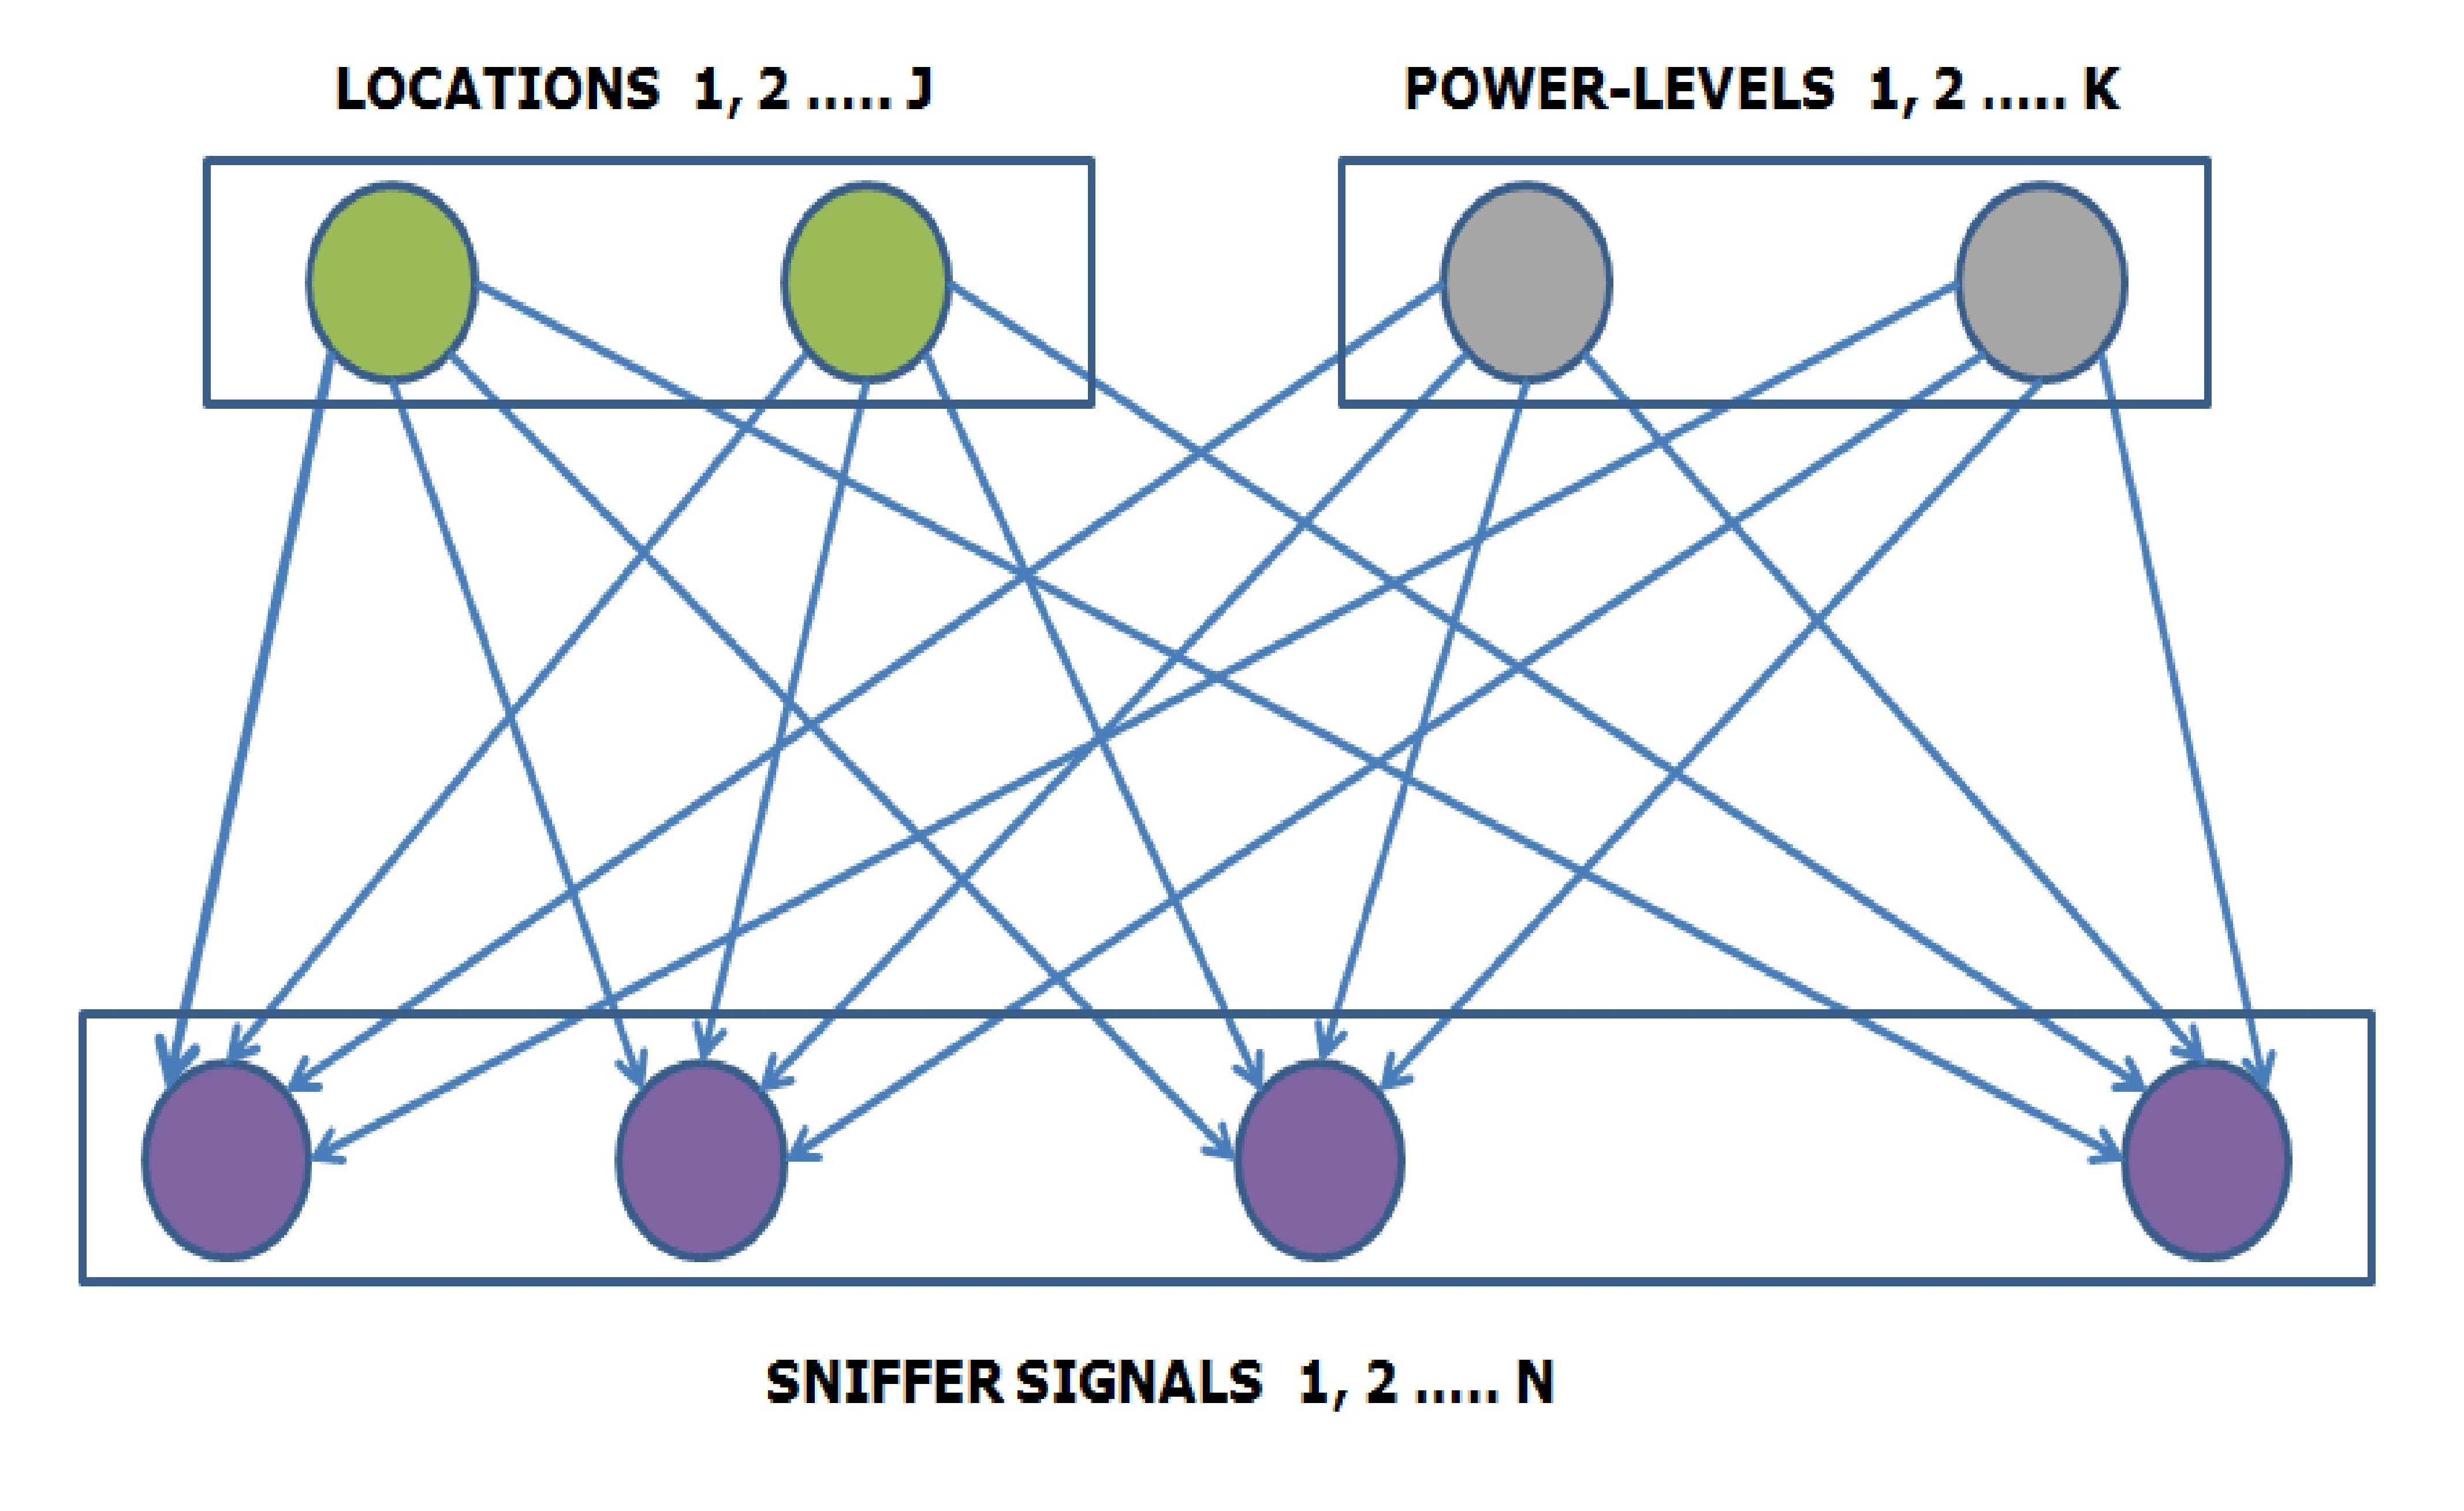
\includegraphics[width=1\textwidth]{Figs4Paper/gmm.eps}
% \caption{The GMM for our problem}
% \label{fig:gmm}
% \end{minipage}%
% \end{figure*}


% \begin{figure*}[h!]
% \begin{minipage}{0.52\textwidth}
% %\subfloat[big]{\label{subfig:a}\includegraphics[width=1\textwidth]{Figs/gaussian.eps}} \\%
% %\subfloat[big2]{\label{subfig:a}\includegraphics[width=1\textwidth]{Figs/gaussian.eps}}%
% 
% \includegraphics[width=1\textwidth]{Figs/gaussian.eps}
% \caption{first minipage}
% \end{minipage}\quad %
% \begin{minipage}{0.33\textwidth}%
% \subfloat[small]{\label{subfig:b}\includegraphics[width=1\textwidth]{Figs/gaussian.eps}}\\%
% \subfloat[small]{\label{subfig:c}\includegraphics[width=1\textwidth]{Figs/gaussian.eps}}%
% \caption{second minipage}
% \end{minipage}%


 %\label{fig:diamond_lattice}
 %\caption{Face-Center-Cubic - \ref{subfig:a}  \ref{subfig:b} \ref{subfig:c} }

%\end{figure*}



% \begin{figure}[h!]
%   \centering
%     \epsfig{file=Figs/gaussian.eps, height=1.5in, width=2.5in}
%   \caption{ Received Signal Strength at a sniffer from a laptop operating at a fixed power-level }
%   \label{fig:gaussian}
% \end{figure}
% 
% \begin{figure}[h!]
% \centering
%   \epsfig{file=Figs/Tx_PowerLevels.eps, height=1.5in, width=2.5in}
%   \caption{Signal strength readings from three different receivers of a signal from a signal transmitter, with the transmitter varying it Tx-Power}
%   \label{fig:txpower}
% \end{figure}

Our system is based on the 802.11 wireless networking protocol, which is
inexpensive and widely deployed in enterprise offices and academic
campuses. 802.11 uses 11 channels in the ISM band. Signal
propagation in this band is complex and in this section, we identify the different
causes of variation in the wireless channel quality and how we factor
them into our model. Our approach is server-based, where we capture
client packets using sniffers. As such, we are mainly concerned with the
variations that affect the Received Signal Strength (RSS) on the
sniffer. In this section, experimentally validate two observations that have been made previously
in wireless-localization literature. We model our problem around these
two observations. 

\subsection{Distribution of Signal Strength}
\label{subsec:distributionofsignalstrength}

\begin{figure} [h!]
\centering
\epsfig{file=Figs4Paper/GaussianDistr/gaussian.eps, height=1.5in, width=2.5in}
\caption{The distribution of RSS observed on a sniffer}
\label{fig:distribution}
\end{figure}


Figure \ref{fig:distribution} shows the distribution of Received Signal
Strength values observed by a sniffer located a fixed distance apart
from a transmitting client. The Tx-client is a Dell laptop having a
Ubiquiti XR2 wireless card and is using a fixed power-level for wireless
transmissions. 

We observe that the Signal Strength distribution is roughly Gaussian. In
\cite{Tao:2003:WLL:941311.941314} Tao et al also make similar observations.
\cite{Haeberlen:2004:PRL:1023720.1023728, Moraes:2006:CWL:1164783.1164799} etc also model signal intensity
as a normal distribution.

\subsection{Transmission Power}
\label{subsec:transmissionpower}

\begin{figure} [h!]
\centering
\epsfig{file=Figs4Paper/TxPower/Tx_PowerLevels.eps, height=1.5in, width=2.5in}
\caption{RSS as a function of the Tx-power of a device.}
\label{fig:txpower}
\end{figure}

Figure \ref{fig:txpower} shows how the observed signal strength changes
as the transmission power is varied. Our experiments validate the
observations made in \cite{Tao:2003:WLL:941311.941314} by Tao et al in that the observed
signal strength is linearly proportional to the transmission power.


\section{Problem Formulation}
\label{sec:problemformulation}

Assume that the target space is discretized into $J$ locations. 
This can be of any level of granularity 
depending on the desired accuracy. Finer granularity does increase computational load, but does not seem to be a bottleneck. There are a set of sniffers or APs doubling as sniffers (a larger number is expected to improve accuracy) that report a vector of RSSs from a target device to be localized to a server that performs the necessary computation. The target device can be static or mobile. In fact, mobility tends to improve performance (more on this later). The location of the sniffers themselves are assumed to be known with respect to which the $J$ locations
are specified. No prior wireless measurements are needed, providing our approach with a significant leverage. 

\subsection{Using Gaussian Mixture Model}
We use the well-known idea of {\em mixture models} in statistics. The idea is to first make a very general assumption that the target could be in any of the $J$ possible locations with varying probabilities. Each of these possibilities can potentially generate a distribution of RSSs
at the set of sniffers. Now, given the vector of RSSs sniffed at the set of sniffers, the problem is to estimate the most likely target 
location out of the $J$ possibilities that could have generated that vector of RSSs. Since 
the same device at the same location but with a different transmit power can generate different distributions of RSSs, an additional subtlety we handle is that the
most likely power level (actually an abstract sense of it) is also
determined as a part of the process. This subtle addition makes the
method adaptive for different devices having their own default power
levels for wireless transmission.

\begin{figure} 
\centering
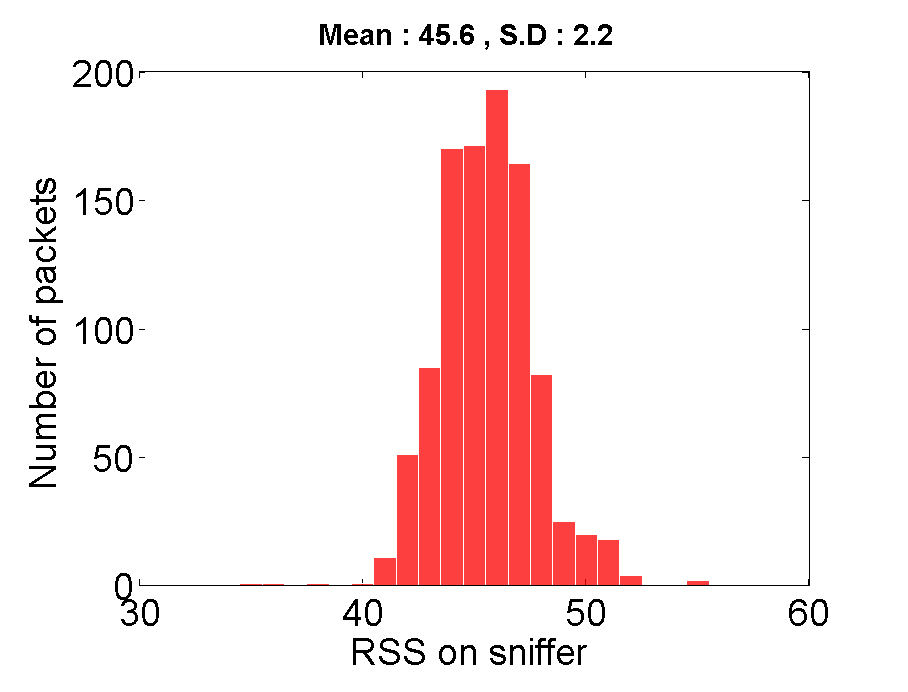
\epsfig{file=Figs4Paper/NewGaussian/distr7.eps, height=1.25in, width=1.6in} 
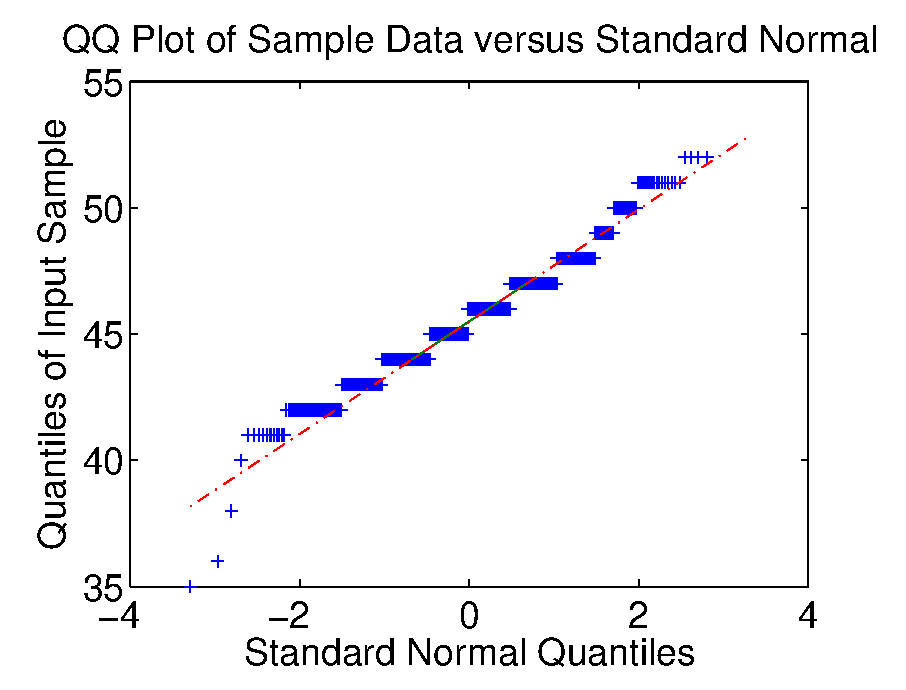
\epsfig{file=Figs4Paper/NewGaussian/qqplot2.eps, height=1.25in, width=1.6in}
\caption{The distribution of RSS observed on a sniffer.}
\label{fig:distribution}
\end{figure}

Before a more formal presentation, a key assumption we must make upfront
is that the distribution of RSS at a sniffer (more specifically an indicator representing RSS, commonly known as RSSI) is Gaussian
given the target device is stationary at a location and transmitting at
a fixed power level. The Gaussian assumption is not uncommon in wireless link modeling~\cite{Haeberlen:2004:PRL:1023720.1023728, Moraes:2006:CWL:1164783.1164799, Tao:2003:WLL:941311.941314}. In fact, the log-normal shadowing model~\cite{Rappaport:2001:WCP:559977} is widely used albeit in a slightly different context. To lend confidence to this assumption on our specific hardware setup, we have performed a set of measurements using the same sniffer and target device hardware used in later experiments. 
Figure~\ref{fig:distribution} shows the measured
RSSI distribution observed on a sniffer in our testbed 
for a stationary client transmitting at a fixed power level. The quality of the Gaussian fit for this distribution is also shown. The fit is very good. 

The Gaussian assumption makes our approach amenable to well-known machine learning tools. Now,
the distribution of the RSSs on the sniffers can be represented by the \emph{Gaussian Mixture Model} or GMM~\cite{Reynolds, Bishop:2006:PRM:1162264} --  a simple linear superposition of Gaussian components. 
Nothing is known a priori about the nature of these Gaussian
and in what proportion they are mixed. They are modeled in terms of discrete latent variables. We describe the modeling approach below.  

\subsection{Latent Variables for Target Locations and Power Levels}
\label{subsec:latentvariablesfortargetlocationsandpowerlevels}

Assume that a $J$-dimensional binary random variable {\bf x} representing possible target locations. $\mathbf{x}$ has a 1-of-$J$ representation in which a particular element $x_{j}$ is equal to one and all other elements are equal to $0$. The values of $x_{j}$ therefore satisfy $x_{j} \in$ \{0,1\} and $\sum_{j} x_{j} = 1$. Thus, there are $J$ possible states for the vector $\mathbf{x}$.

The probability distribution over $\mathbf{x}$ can be specified as a multinomial 
\begin{align}
 p(x_{j} = 1) = \upsilon_{j},
\end{align}
where the parameters $\{\upsilon_{j}\}$ must satisfy
\begin{align}
0 \le \upsilon_{j} \le 1 \ \text{and} \ \sum_{j=0}^{J} \upsilon_{j} = 1.
\end{align}

Similarly, assume that a $K$-dimensional binary random variable $\mathbf{z}$ representing Power Levels. $\mathbf{z}$ has a 1-of-$K$ representation in which a particular element $z_{k}$ is equal to 1 and all other elements are equal to 0. The values of $z_{k}$ therefore satisfy $z_{k} \in$ \{0,1\} and $\sum_{k} z_{k} = 1$. Vector {\bf z} has $K$ possible states.

The distribution over $\mathbf{z}$ is specified as a multinomial 
\begin{align}
p(z_{k} = 1) = \tau_{k},
\end{align}
where the parameters $\{\tau_{k}\}$ must satisfy
\begin{align}
0 \le \tau_{k} \le 1 \ \text{and} \  \sum_{k=0}^{K} \tau_{k} = 1.
\end{align}


\begin{figure} [h!]
\centering
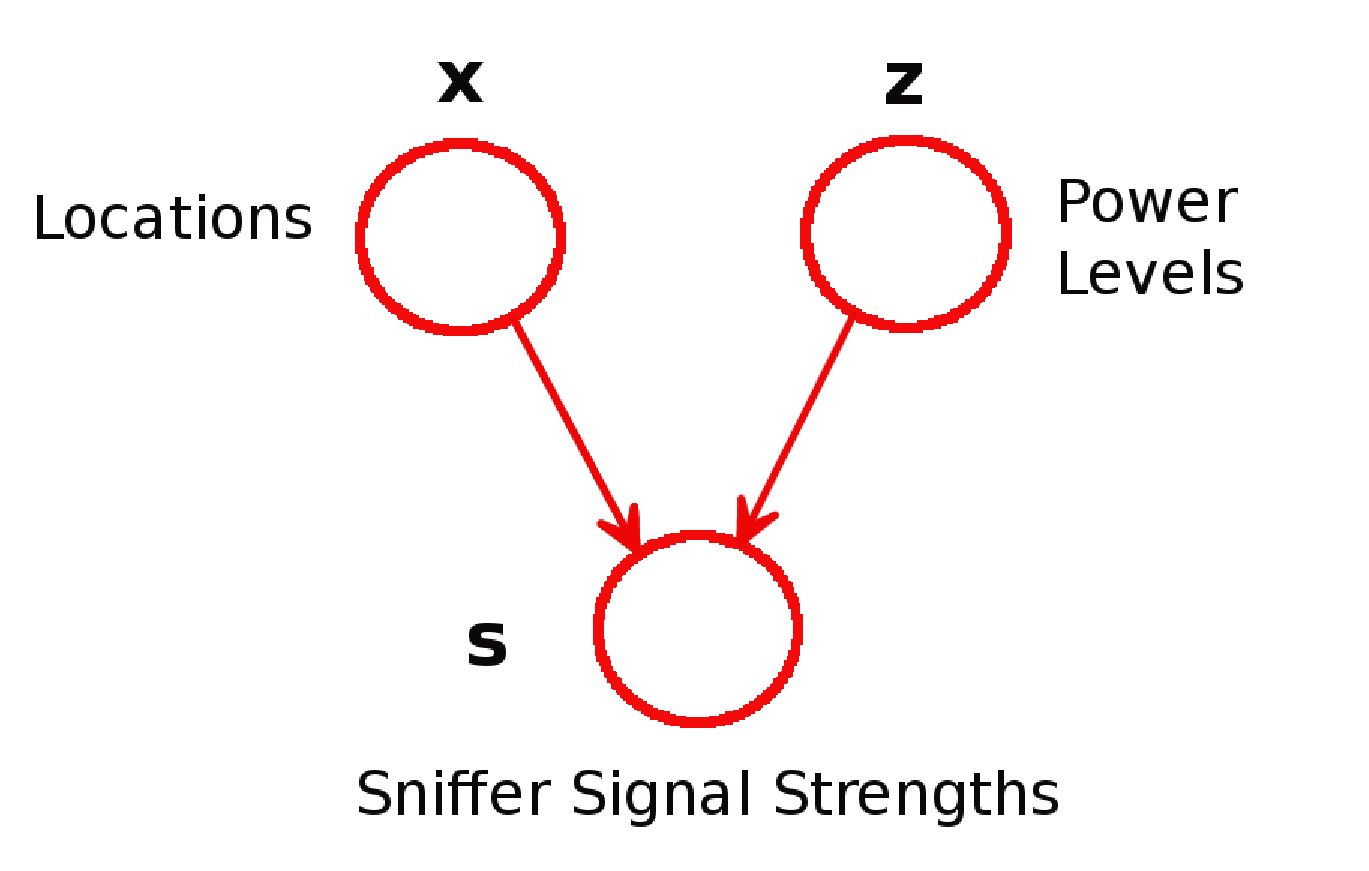
\epsfig{file=Figs4Paper/GMM/gmm4.eps, height=1.5in, width=2.5in}
\caption{The GMM for our problem.}
\label{fig:gmm}
\end{figure}


\subsection{RSSI Distribution}
\label{subsec:constructingthedistributionovertheobservedsignalstrengths}

Let $\mathbf{s}$ be the $N$-dimensional vector representing the RSSI observed by the $N$ sniffers in the target area. 
Using the chain rule of probability, we can now define the joint distribution $p(\mathbf{s}, \mathbf{x},\mathbf{z})$ in terms of the distribution $p(\mathbf{x},\mathbf{z})$ and the conditional distribution $p( {\bf s} | {\bf x}, {\bf z})$, 
corresponding to the graphical model in Figure \ref{fig:gmm}:
\begin{align}
p( {\bf s}, {\bf x}, {\bf z}) &= p( {\bf x}, {\bf z}) p( {\bf s} | {\bf x}, {\bf z}).
\end{align}
Since {\bf x} and {\bf z} are independent random variables,
\begin{align}
p( {\bf s}, {\bf x}, {\bf z}) &= p( {\bf x}, {\bf z}) p( {\bf s} | {\bf x}, {\bf z}) \nonumber \\
&= p({\bf x})p({\bf z})p( {\bf s} | {\bf x}, {\bf z}). \label{eqn:joint_distribution}
\end{align}

Equation \ref{eqn:joint_distribution} gives us the joint distribution of $ p( {\bf s}, {\bf x}, {\bf z}) $. The marginal distribution of {\bf s} is then obtained by summing the joint distribution over all possible states of {\bf x} and {\bf z}:
\begin{align}
p( {\bf s}) & = \sum_{\bf x}\sum_{\bf z} p({\bf x})p({\bf z})p({\bf s}|{\bf x}, {\bf z}).\label{eqn:marginal_distribution1}
\end{align}

%\subsubsection{Independence of Sniffers}
%\label{subsubsec:independenceofsniffers}

Now assume that the RSSIs observed at different sniffers are independent. This is justified as the sniffers are typically at disparate locations and thus the wireless propagation path loss can be assumed independent. 
Thus, the term $p( {\bf s} | {\bf x}, {\bf z})$ in equation
\ref{eqn:marginal_distribution1} can be simplified as
\begin{align}
p( {\bf s} | {\bf x}, {\bf z}) & = \prod_{i=1}^N p({s_{i}} | {\bf x}, {\bf
		z}). \label{eqn:conditional_distribution1}
\end{align}
Based on the Gaussian assumption made before, the RSSI can be modeled 
as Gaussian random variables determined by the (location, power-level) pair, so that
\begin{align}
s_{i} | {x_{j}=1}, {z_{k}=1}  \sim  \text{Gaussian}(\mu_{i, (j,k)}, \sigma_{i, (j,k)}).
\end{align}
This lends simplicity to our model since the term $p( {\bf s} | {\bf x}, {\bf z})$ in equation
\ref{eqn:conditional_distribution1} can be expressed succinctly as 
\begin{align}
p( {\bf s} | {\bf x}, {\bf z}) & =  \prod_{j=1}^J \prod_{k=1}^K 
		\prod_{i=1}^N \mathcal{N}(s_{i} |  \mu_{i, (j,k))},\sigma_{i, (j,k)}^2)^{x_j z_k} \, . \label{eqn:conditional_distribution2}
\end{align}
Note that for any given ${\bf x}$ and ${\bf z}$ only one term in the product is actually active for all $i$, because the exponent $x_j z_k$ acts as a selector: $x_j z_k = 1$ for exactly one index pair $(j,k)$, and equals $0$ for all others.

From now on, for notational convenience we define
\[
\mathcal{N}(\mathbf{s} |  \boldsymbol\mu_{(j,k))},\boldsymbol\sigma_{(j,k)}^2) \equiv \prod_{i=1}^N \mathcal{N}(s_{i} |  \mu_{i, (j,k))},\sigma_{i, (j,k)}^2) \, . 
\]

\subsection{Model Parameters}
\label{subsec:modelparameters}

Putting equations \ref{eqn:marginal_distribution1} and
\ref{eqn:conditional_distribution2} together we get the marginal probability distribution over
{\bf s} as
\begin{align}
p( {\bf s}) &= \sum_{j=1}^J \sum_{k=1}^K \upsilon_{j} \tau_{k} \mathcal{N}(\mathbf{s} |  \boldsymbol\mu_{(j,k))},\boldsymbol\sigma_{(j,k)}^2) \, .
\end{align}

Thus we have modeled the marginal distribution of {\bf s} as a Gaussian
mixture with target locations and power levels as the latent variables. The parameters of the model are 
\begin{align}
{\boldsymbol\theta} = \left( {\boldsymbol\upsilon} , {\boldsymbol\tau},  {\boldsymbol\mu} , {\boldsymbol\sigma}^2\right)\, .
\end{align}

Henceforth, we refer to this model as {\bf WiGMM}. We now use the widely popular \emph{Expectation-Maximization} (EM) algorithm~\cite{Dempster77maximumlikelihood, Borman_theexpectation, Bilmes97agentle, DinovIvoD, Bishop:2006:PRM:1162264} to estimate the parameters of the model.

\section{EM Algorithm}
\label{sec:emalgorithm}

An elegant and powerful method for finding maximum likelihood solutions
for models with latent variables is the \emph{Expectation Maximization} 
	algorithm. The EM algorithm is an iterative process through two
	steps: an expectation step (E-step) and a maximization step (M-step). During the iterations, a sequence of model parameters ${\bf \theta^{0}}$
, ${\bf \theta^{1}}$, ...., ${\bf \theta^{*}}$ is generated where ${\bf \theta^{0}}$ is the initial parameter and ${\bf \theta^{*}}$ is the converged parameter when the algorithm terminates.

\subsection{E-step}
\label{subsec:estep}

Suppose we have a data set of RSSI observations at
the sniffers from the target device: ${\bf \overline{S}}$ = \{
${\bf {s}}^{0}$, ${\bf {s}}^{1}$,\ldots,${\bf {s}}^{M}$\}. The E-step
corresponds to finding the expected value of the latent or hidden component ({\bf
		x} and {\bf z}) values given the observed data  ${\bf \overline{S}}$ and the current parameter estimates.
Using this observation set and the current parameter estimates, we find out the posterior probabilities \textbf{(or responsibilities)} as follows. 
For each observation ${\bf {s}}^{l}$,
\begin{align}
& \pi_{({x_{j}}, {z_{k}})}^{l}  = p({x_{j}} = 1, {z_{k}} = 1 | {\bf{s}}^{l}) \\ 
& = \frac { p({x_{j}} = 1)p({z_{k}} = 1)p( {\bf {s}}^{l} | {x_{j}} = 1, {z_{k}} = 1)} {\ \sum_{p=1}^J \ \sum_{q=1}^{K} p({x_{p}} = 1) p({z_{q}} = 1) p( {\bf {s}}^{l} | {x_{p}} = 1, {z_{q}} = 1)} \nonumber \\ 
& = \frac { \upsilon_{j} \ \tau_{k} N({\bf {s}}^{l} | {\bf {\mu}}_{j,k}, {\bf {\sigma}}_{j,k})} {\sum_{p=1}^J \sum_{q=1}^K \left[\upsilon_{p} \tau_{q} N({\bf {s}}^{l} | {\bf {\mu}}_{p,q}, {\bf {\sigma}}_{p,q})\right]. } 
\end{align}

\noindent The posterior probability value $\pi_{({x_{j}}, {z_{k}})}^{l}$ can be viewed as the {\it responsibility} that component $({x_{j}}, {z_{k}})$ takes for explaining observation ${\bf {s}}^{l}$. We determine this measure of responsibility for each observation in the data set ${\bf \overline{S}}$.

\subsection{M-step}
\label{subsec:mstep}

The M-step of the algorithm corresponds to `maximizing the likelihood' of
the observed data. This leads us to re-estimating the parameters for the next iteration based on the posterior probabilities calculated in the expectation step of the algorithm:
\begin{align}
\upsilon_{j} = \frac { \sum_{l=1}^{M} \ \sum_{k} \pi_{({x_{j}}, {z_{k}})}^{l}} {M},
\end{align}
\begin{align}
\tau_{k} = \frac { \sum_{l=1}^{M} \ \sum_{j} \pi_{({x_{j}}, {z_{k}})}^{l}} {M},
\end{align}
\begin{align}
\mu_{i \ (j,k)} = \frac  { \sum_{l=1}^{M} \pi_{({x_{j}}, {z_{k}})}^{l} s_{i}^{l}} {N_{j,k}},
\end{align}
where
\begin{align}
{N_{j,k}} = \sum_{l=1}^{M} \pi_{({x_{j}}, {z_{k}})}^{l}.
\end{align}

The variance parameter can also be updated accordingly.

\subsection{Convergence of Log Likelihood}
\label{subsec:convergenceofloglikelihood}

\begin{figure}
\centering
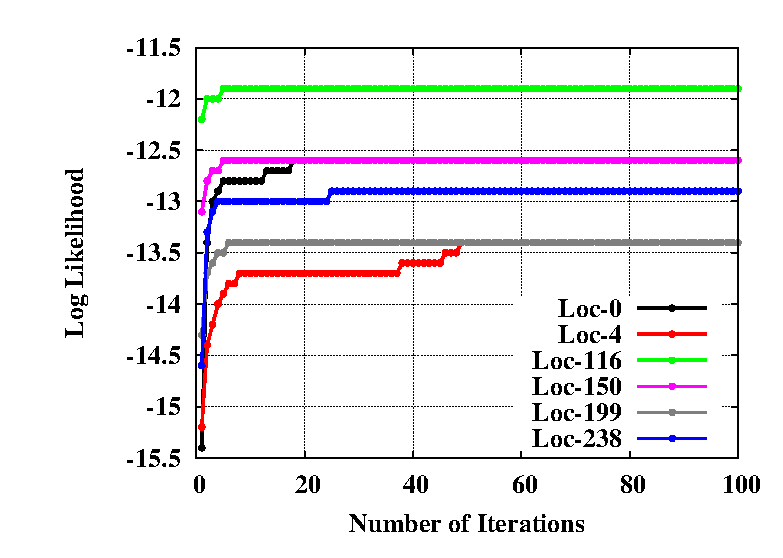
\epsfig{file=Figs4Paper/CEWIT/GMM-LogLikelihood/LogLikelihood.eps, height=1.5in, width=2.5in}
\caption{Convergence of log likelihood for 6 different instances of using GEM.}
\label{fig:loglikelihood}
\end{figure}

Each update of the parameters resulting from an E-step followed by an
M-step is guaranteed to increase the log likelihood function:
\begin{align}
\ln p({\bf \overline{S}} | {\bf \theta}) &= \sum_{l=1}^{M} \ln \left\{
\sum_{j=1}^J \sum_{k=1}^K \upsilon_{j} \tau_{k} \mathcal N ({{\bf {s}}^{l}} | {{\bf {\mu}}_{j,k}}, {{\bf \sigma}_{j,k}})\right\}.
\end{align}
The algorithm is deemed to have converged when the change in the log likelihood function falls below a threshold ($10^{-6}$ in the experiments described later).
Figure \ref{fig:loglikelihood} shows how the log-likelihood converges for six different instances of running GEM. Each instance here was to localize an android phone on the CEWIT testbed.



\subsection{Handling Identifiability}
\label{subsec:handlingidentifiabilityinourmodel}

There is an identifiability problem in this general approach that is well understood~\cite{Bishop:2006:PRM:1162264}. This arises because there are $P!$ equivalent solutions
in a $P$ component mixture model. In our case,
each component is a (location,
power-level) pair. 
We handle the problem of identifiability 
by using the knowledge of sniffer locations and initializing the EM algorithm
using the basic log-distance radio propagation model~\cite{Rappaport:2001:WCP:559977, Molkdar91} below:
%\subsubsection{Indoor Radio Propagation Model}
%\label{subsubsec:indoorradiopropagationmodel}
\begin{align}
P_r(d) = G\frac{P_t}{d^\alpha},
\end{align}
where $P_r(d)$ is the received power at distance $d$ and $P_t$ is the transmit power.
$\alpha$ is the path loss exponent which is simply a model parameter. 
In free space $\alpha =2$, but it typically increases somewhat in complex 
environments. $G$ is a frequency and antenna dependent constant. 
Often the above equation is expressed somewhat differently as: 
\begin{align}
P_r(d) = P_r({d_0}) - 10\alpha\log\left(\frac {\it d} {\it d_{0}}\right)
	\label{eqn:pathloss_1},
\end{align}
%\noindent
where $P_r$ is now expressed decibel (dB) units. This emphasizes that when powers 
are expressed in dB units
transmit power changes expressed in dB causes the same dB change at all receivers
regardless of location. In our experiments we will use RSSI in dB units. We independently
verified (not reported here for brevity) that the RSS measurement on our sniffer hardware is accurate at least to the extent
that a dB shift in the transmit power does get recorded as a similar
shift at the sniffer regardless of location.

\subsubsection{Initializing the components of our Model}
\label{subsubsec:initializingthecomponentsofourmodel}

In Equation \ref{eqn:pathloss_1},  $P_r({d_0})$ is the signal power at
some reference distance $d_{0}$ from the sniffer. This reference signal
strength $P_r({d_0})$ can be derived empirically or obtained from
wireless network hardware specifications \cite{Bahl00radar:an}. In our
deployment all our sniffers have the same hardware (described in detail
		in Section \ref {sec:evaluation} ) . The value of $P_r({d_0})$
was empirically found to be approximately 60 dB when $d_{0}$ = 1 meter . No assumption is made about the
target space, so $\alpha =2$. The path loss equation of equation
\ref{eqn:pathloss_1} can now be succintly expressed as: 
\begin{align}
P_r(d) = 60 - 10\alpha\log\left({\it d} \right)
	\label{eqn:pathloss_2},
\end{align}
 
For a location $L$ at a distance $d$ from a sniffer, equation
\ref{eqn:pathloss_2} gives us the theoretical RSSI value $P$ at the
sniffer. However, different devices may work at different power-levels
for doing wireless transmissions. Thus we generate $k$ values ranging from
$[P-\frac{k}{2} , P+\frac{k}{2}]$ to initialize the means for the $k$
component from location $L$. We do this procedure for every possible
target location in the map.  The standard deviation ($\sigma_{j, k}$)
	was chosen as 5 (and kept fixed to reduce computation time). This
	choice was mostly arbitrary though some previous work
	\cite{Tao:2003:WLL:941311.941314} also use fixed values of standard
	deviation ($\sigma=12$) in
	their work. 

\subsection{Final Location Estimate}
\label{subsec:finallocationestimate}

\begin{figure*}
	\centering
		\subfloat[CEWIT]{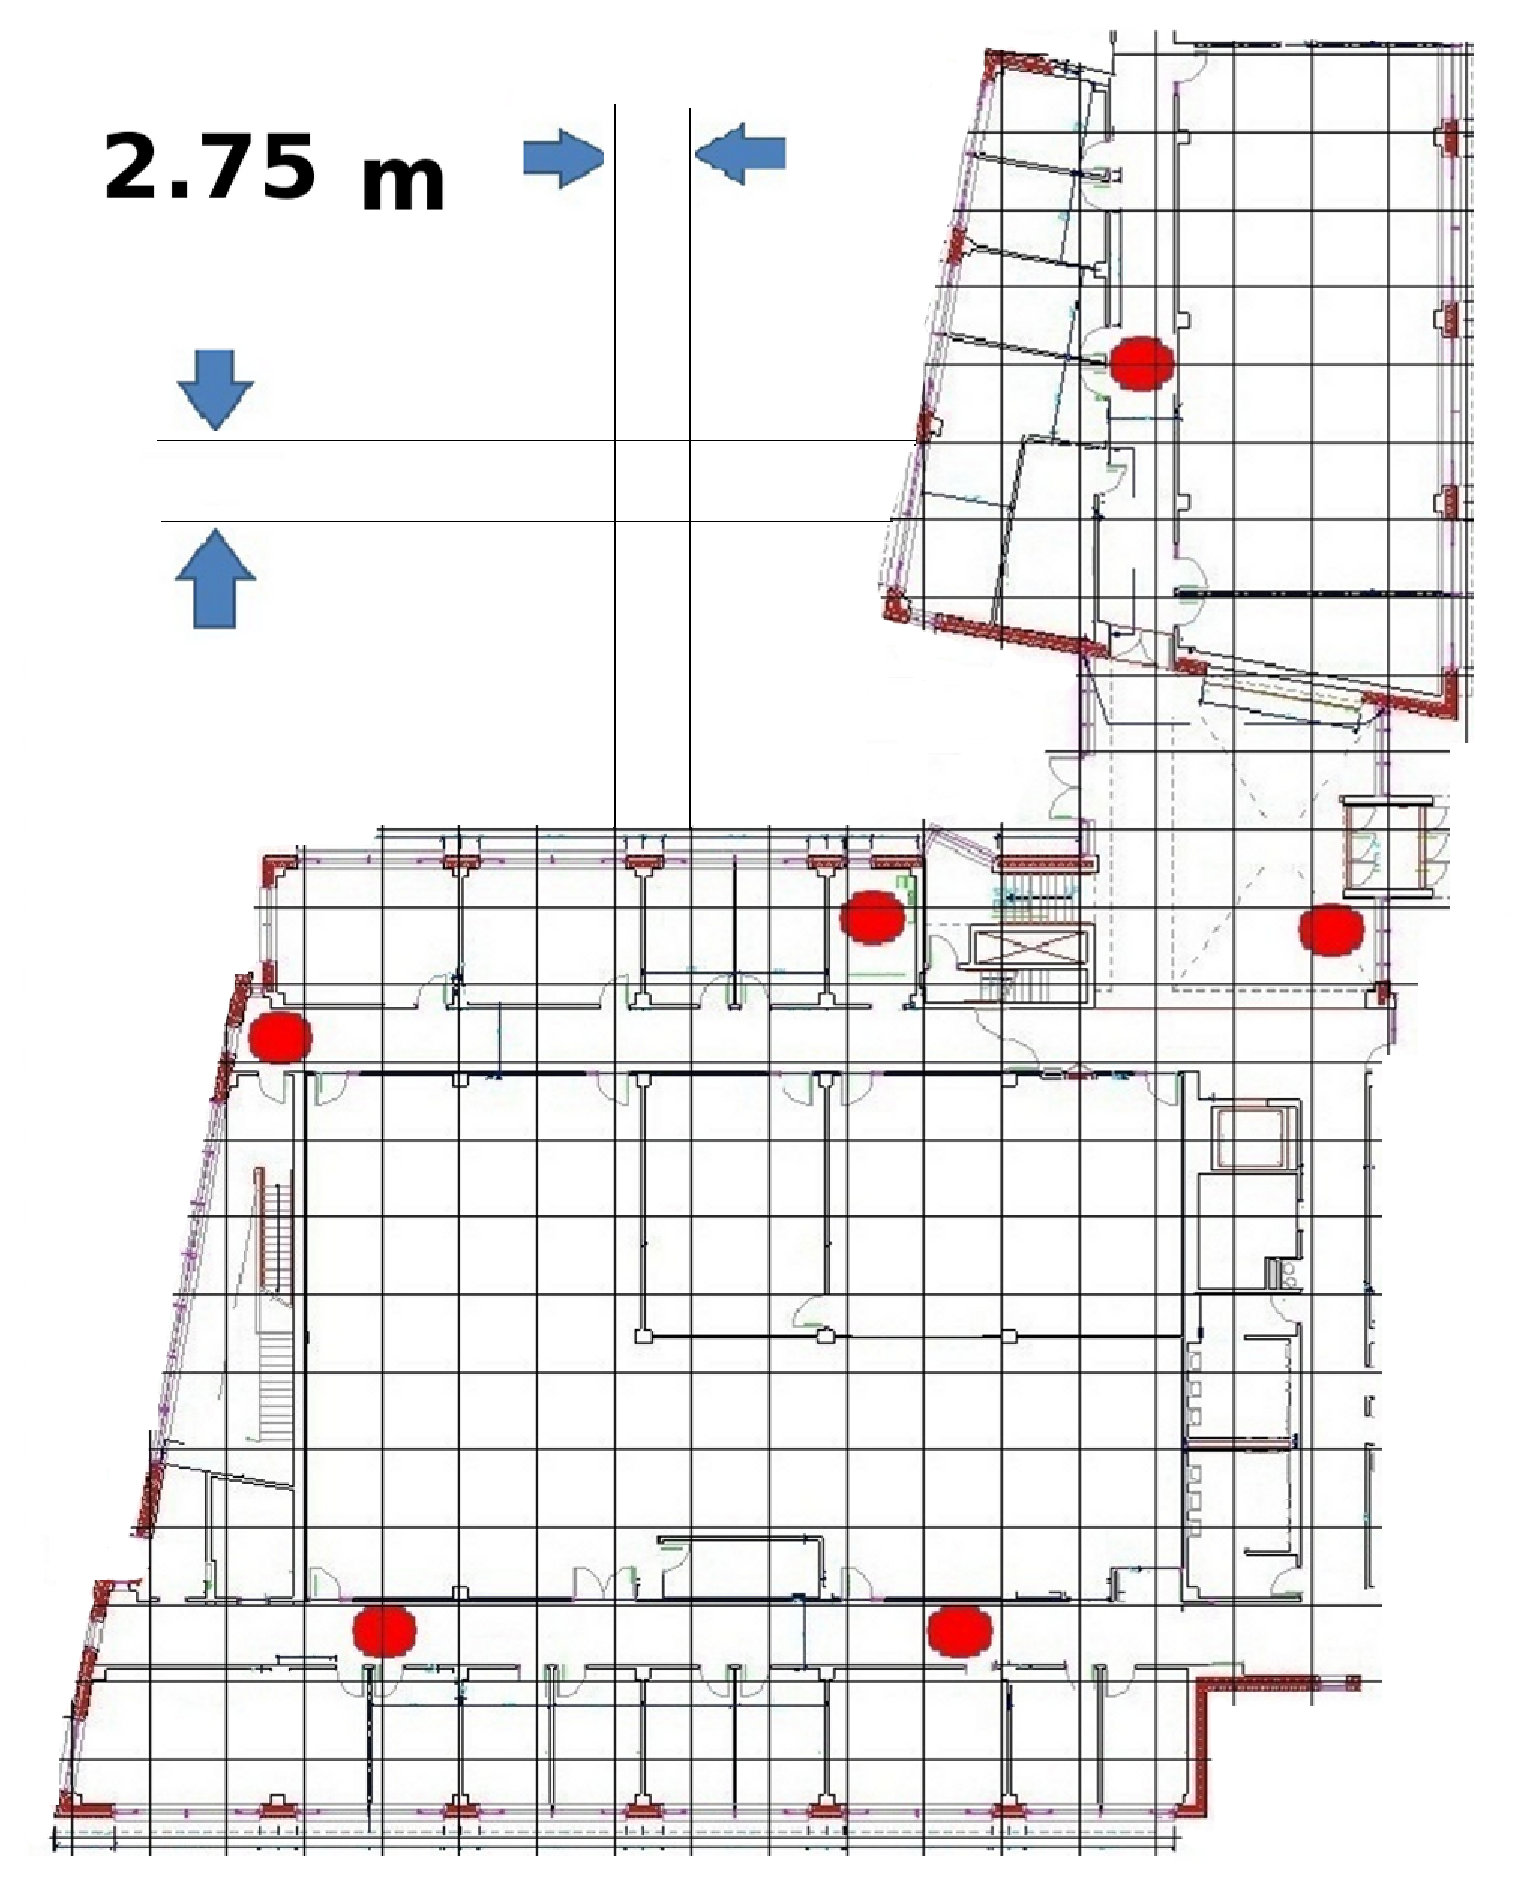
\includegraphics[height=2.5in, width=2in]{Figs4Paper/CEWIT/CEWIT-Map7.eps}} \quad \quad
		\subfloat[CSD]{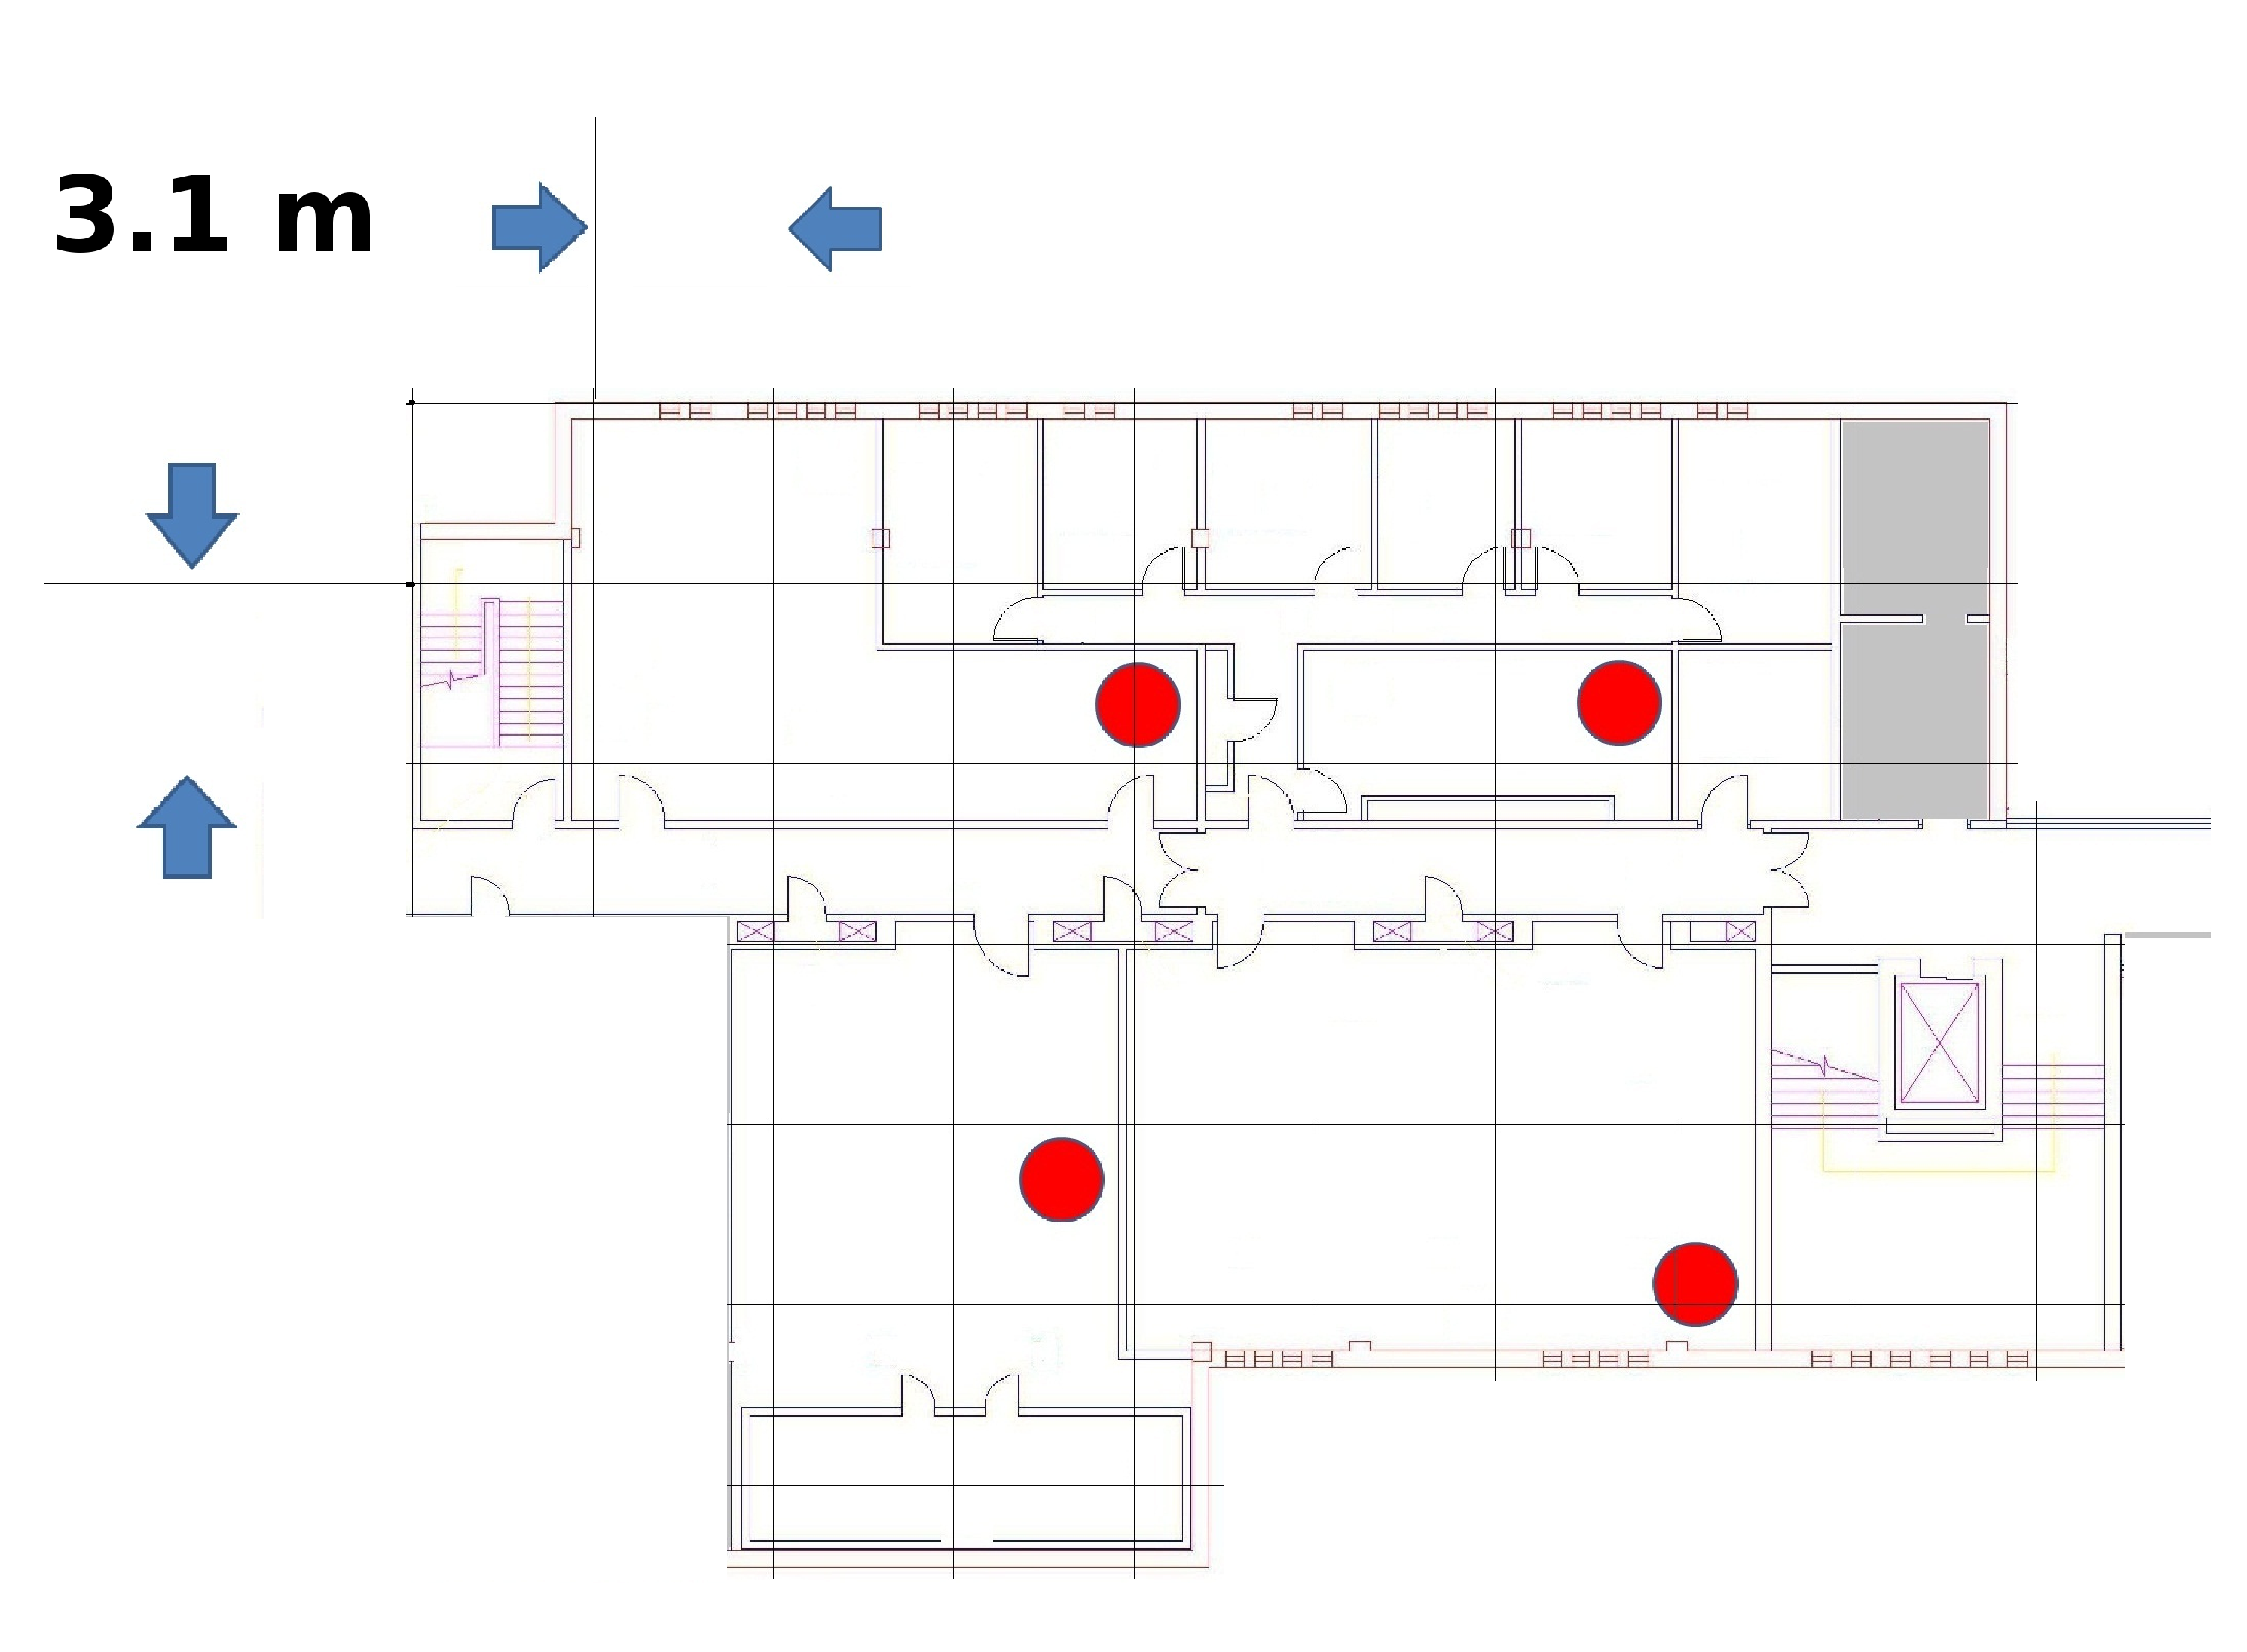
\includegraphics[height=1.5in, width=2.5in]{Figs4Paper/CSD/CSD-Map4.eps}} 
	\caption{Two testbeds for validation experiments. The red circles represent sniffer locations.}
	\label{fig:experimenttestbed}
\end{figure*}


Given a real-time received RSS vector ${\bf {s}}^{(obs)}$, we can now
find the location with the highest probability. We do this by first
finding the probability for each (location, power-level) pair and then
marginalizing over the power-levels. This gives us a probability
distribution over the possible locations inside the target space. The
location with the highest probability is returned as the answer.
Thus the estimated location index is given by $j^{*}$ where
\begin{align}
j^{*} = max_{j} \sum_{k} P({x_{j}} = 1, {z_{k}} = 1 | {\bf {s}}^{(obs)}) 
\end{align}

\section{Experiment Methodology}
\label{sec:experimentmethodology}

We start with a description of our system setup, including an overview of the components of our sniffer devices. We then present details about the two testbeds where we conducted our experiments. Finally, we round up this section by discussing the data collection process.

\subsection{System Setup}
\label{subsec:systemsetup}

As mentioned briefly in Section \ref{sec:introduction}, GEM uses an infrastructure based
architecture. The system has two main components: stationary sniffer devices in the target space and a centralized server running the GEM algorithm. Sniffers provide overlapping coverage of the target area (similar to WLAN APs). The server notifies the sniffers about the MAC id of the target device, the channel number and the listening period. The sniffers then record the RSSI of all packets received that match the server's query. The recorded information is sent to the server which then makes a location estimation using the GEM algorithm.

In the current prototype, the server communicates with the sniffer devices using in-building power-line network. In the ultimate embodiment, the sniffer functionality could be integrated directly into the WLAN APs. If necessary and appropriate, a localization application can also run on the client that downloads the building map as soon as gets connected to the WLAN, sends a localization request to the WLAN and shows the location on the map. 

\subsubsection{Sniffer Information}
\label{subsec:snifferinformation}

%The sniffer devices are responsible for capturing wireless transmissions made by a Tx-client. 

We use Soekris net4801~\cite{} SBCs as sniffer
devices with atheros-based CM9 cards for wireless captures. The sniffers run Pyramid Linux (version 2.6.16-metrix). The default
MadWiFi driver is used comes with this distribution (0.9.4.5:svn 1485). 

To capture packets the standard Tcpdump tool (version 4.0.0/libpcap version 0.9.8) is used. To obtain signal strength information, the MadWiFi driver allows a
monitor mode interface to be created and configured with the radio tap header support. 
The radio tap header reports the SNR (in dB) as the RSSI. This is what we use directly. 
Since the noise floor reported by the cards is constant (-95dBm), the RSSI value 
is also the same as the RSS (in dBm) with a constant difference. 

%ra header we can extract the
%RSSI of each packet received by the sniffer. We verified that the MadWifi driver had a fixed noise-floor in each of our
%cm9 cards (-95 dbm). In fact the received signal strength of a frame reported by the MadWiFi driver is actually the SNR value (in db) obtained after subtracting the noise-floor from the raw signal strength value. We work directly with the RSSI value (in db) as reported by the driver.

\begin{figure*}
	\centering
		\subfloat[CEWIT]{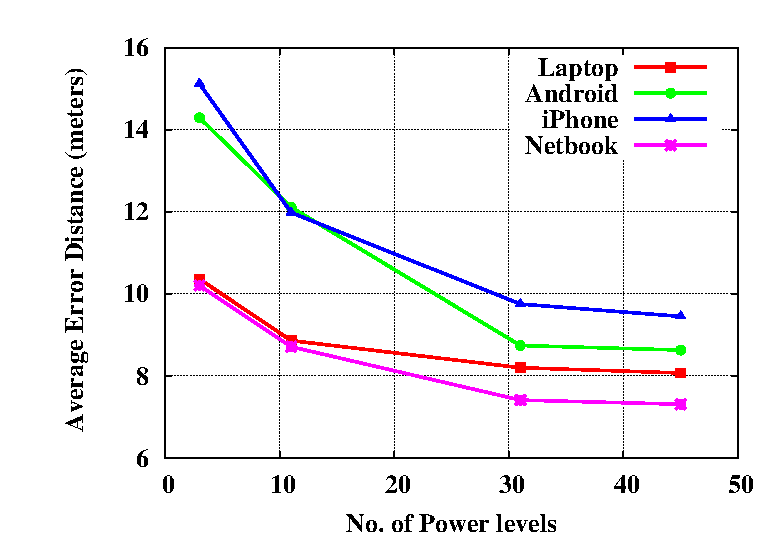
\includegraphics[height=1.5in, width=2.5in]{Figs4Paper/CEWIT/PowerPlot4Paper_CEWIT/PwrLvlPlot_cewit.eps}}
		\subfloat[CSD]{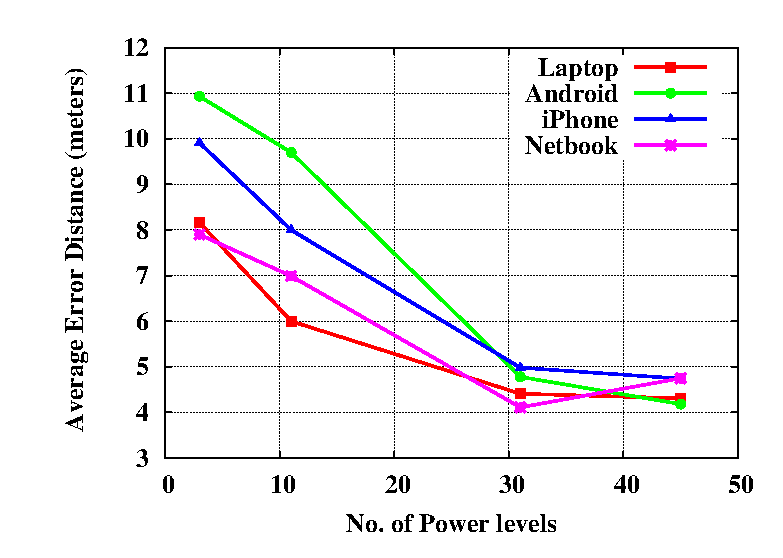
\includegraphics[height=1.5in, width=2.5in]{Figs4Paper/CSD/PowerPlot4Paper_CSD/PwrLvlPlot_csd.eps}}
	\caption{Avg Error distance as a function of the number of power levels}
	\label{fig:powerlevelsvserrordistance}
\end{figure*}

\subsection{Testbed Details}
\label{subsec:testbeddetails}

Two different indoor testbeds are used for validation. The first building, henceforth called CEWIT, is a research and development center in the university with a dimension of 65 meter $\times$ 50  meter. The L-shaped floor comprises of several obstructions in the form of walls of various types, glass and metal doors, office furnitures, server-rack cabinets etc. The second, building henceforth called CSD, is part of the building housing the computer science department. See Figure~\ref{fig:experimenttestbed}. This rectangular-shaped floor has a dimension of 20 meter $\times$ 30 meter and also have walls and various partitions and office furnitures. Both these testbeds had a continuous flux of people moving around in the building at the time
the experiments were conducted. The CEWIT and CSD testbeds use 6 and 4 sniffers respectively. 
See Figure~\ref{fig:experimenttestbed} for the sniffer locations. 

\subsection{Data Collection Methodology}
\label{subsec:datacollectionmethodology}

The CEWIT testbed is discretized into 45 distinct locations roughly every 5.5 meters. The CSD testbed is divided into 27 distinct locations roughly every 3.3 meters. See Figure~\ref{fig:experimenttestbed}. Multiple device types are used. For each device, we transmit 200 ping packets from every distinct location of the corresponding testbed. This is typically accomplished by having 
the user hold the mobile device and walk across the floor of the building briefly stopping at each marked location to transmit 200 ping packets. The ground truth is noted at each location before moving on to the new location. Note that the ground truth information is used only for evaluation of the localization error and is not supplied to GEM for training. Each ping packet is separated uniformly apart at a rate of 1 per second. On the server, the sequence number in the ping packet is used to form the vector of RSSI values recorded by individual sniffers for each transmission. Thus, from each distinct location on the map and for each device type, we have a set of 200 RSSI tuples. This comprises our entire data set that we use in this paper. Experiments on RADAR and Probabilistic (described later in this paper) use a subset of this dataset for building the RF signal map and the remainder data for calculating localization error. 

\subsubsection{Test Devices}
\label{subsubsec:testdevices}

Four different wireless devices are used - a laptop, an android phone, an iphone, a netbook. The laptop is a Dell Inspiron 1545 running Ubuntu v9.04. The android phone is a Google Nexus One. An iphone 3GS (iOS version 4.2.1) is also used. The netbook used is a Dell Latitude 2110 running Ubuntu v9.10. Each device is using its default driver and default power levels for WiFi transmissions. %The devices are henceforth referred to as {\it Laptop}, {\it Android}, {\it iPhone} and {\it Netbook} respectively. 
The data is collected over a span of several days. The devices are not oriented
in any specific direction while making the ping transmissions. The orientation is simply left to the user's choice or convenience. 

%\subsubsection{Sniffer Position}
%\label{subsubsec:snifferposition}
%
%The CEWIT and CSD testbeds have six and four sniffers respectively. See Figure \ref{fig:experimenttestbed}. We assume knowledge of the sniffer positions in the map and use this information to calculate the signal strength values given by the indoor radio propagation model (Equation \ref{eqn:pathloss_2}). These values are used to initialize our algorithm as explained in Section \ref{subsec:handlingidentifiabilityinourmodel} .

\section{Evaluation}
\label{sec:evaluation}

In this section, we present a comprehensive overview of our experimental results. We evaluate the performance of GEM on our two experimental testbeds. We attempt to answer the following questions :

\begin{itemize}

\item What is the number of power-levels that we should use in GEM i.e what is the value of K (mentioned in Section \ref{subsec:latentvariablesfortargetlocationsandpowerlevels} above) that we should use when we run GEM on the back end localization server. 
\item How does the localization accuracy vary as the size of the learning data-set increases.
\item GEM accuracy for heterogenous devices with unmodelled hardware and power-level characteristics
\item How does GEM perform with respect to a model-based scheme that uses the indoor radio path loss propagation model. This presents a true head-to-head comparison because both the techniques do not need pre-deployment effort and can work on the same granularity of discretization of the target space.
\item How does GEM perform with respect to schemes that build RF signal maps like RADAR and Probabilistic. This experiment shows how the WiFi hardware variance problem can impact the accuracy of RF signal map schemes and also show the impact of training granularity for signal map based schemes.
\item We also study how the mobility of a client can actually improve GEM's localization accuracy. 

\end{itemize}

\subsection{Number of powers levels to use in GEM}
\label{subsec:numberofpowerlevelstouseingem}

As mentioned in Section \ref{subsec:datacollectionmethodology} above, the CEWIT testbed has 45 distinct locations and CSD has 27 distinct locations, and for each distinct location on the map and for each device type we have a set of 200 RSS tuples. We divide these 200 tuples into two sets of 100 tuples each: one for learning the GEM parameters and the other for testing the GEM localization results. Each device type is considered separately. Figure \ref{fig:powerlevelsvserrordistance} shows the results of the average error distance (in meters) for the four devices across varying number of power levels used in GEM. We see that the average error distance hits a plateau after K = 31. This is an interesting result because it helps us bound the number of power levels to use. We use a value of K = 45 in the subsequent experiments. 

\subsection{Localization accuracy as a function of the learning set size in GEM}
\label{subsec:localizationaccuracyasafunctionofthelearningsetsizeingem}

\begin{figure}[h!]
\centering
  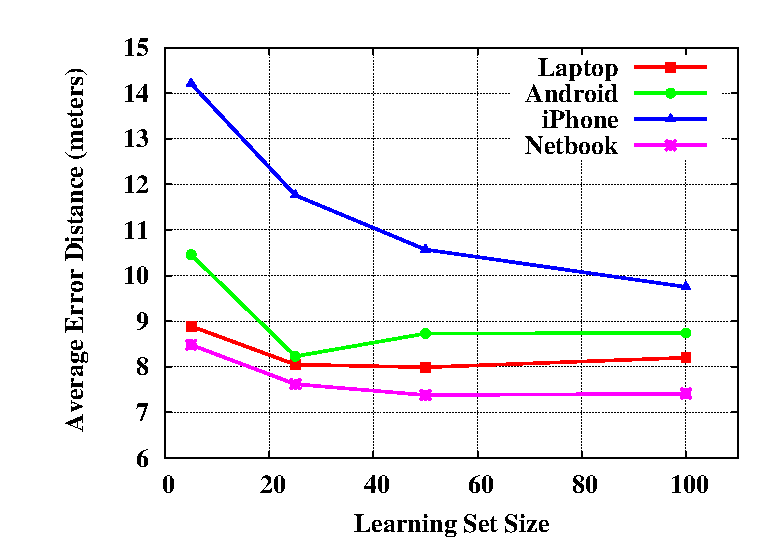
\epsfig{file=Figs4Paper/CEWIT/LearningSize4Paper_CEWIT/LearningSetSize_cewit.eps, height=1.5in, width=2.5in}
  \caption{Average Error distance on the CEWIT Dataset as a function of the learning set size}
  \label{fig:learningsetsizevserrordistance}
\end{figure}

Having fixed the number of power levels to use, we now study how the size of the learning data-set changes the average error distance. Recollect here that as part of our data collection methodology, we have 200 RSS tuples for every location on the map for each of the four device types. This time we again divide the 200 tuples into two sets : one set for learning and the other for testing. The test set size is kept fixed at 100 RSS tuples. From the remaining tuples, the learning set size is varied from 2 tuples going up to 100 tuples. Each device type is considered separately. Figure \ref{fig:learningsetsizevserrordistance} shows the results of the average error distance (in meters) in the CEWIT testbed as the size of the learning set varies. We observe that for all the four devices, the average error does not vary much as the as we move from 50 training samples to 100 training samples. The CSD testbed results (not included here) converged after 25 training samples itself. The experiments which follow have been done keeping the GEM learning set size at 100 and using the remaining 100 samples for testing the localization accuracy.  

\subsection{GEM accuracy for heterogeneous devices}
\label{subsec:gemaccuracyforheterogeneousdevices}

\begin{figure*}
	\centering
	      \subfloat[CEWIT]{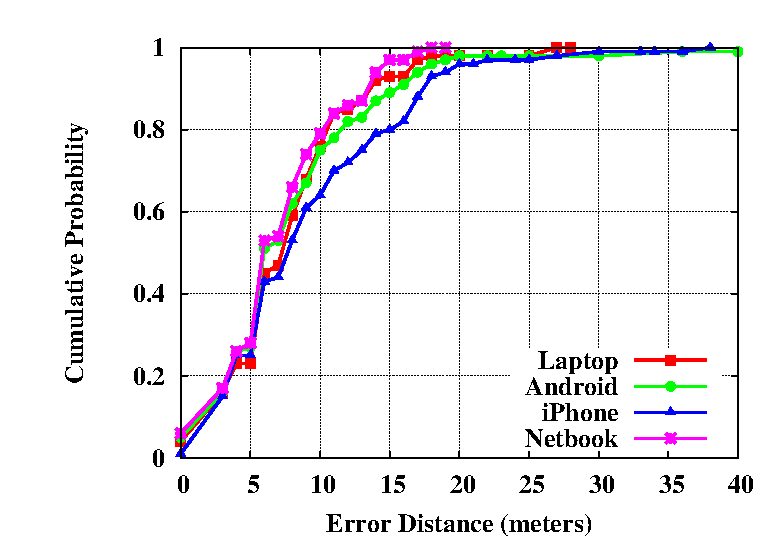
\includegraphics[height=1.5in, width=2.5in]{Figs4Paper/CEWIT/Gem4Devices_CEWIT/4Devices_cewit.eps}}
	      \subfloat[CSD]{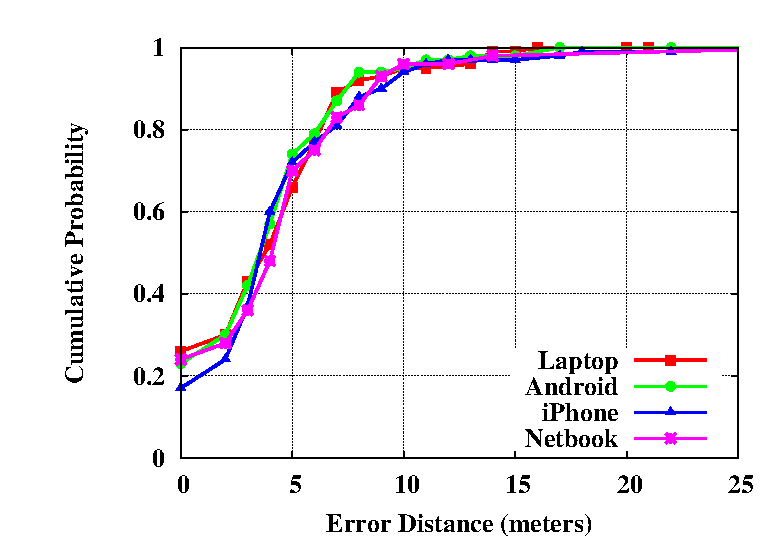
\includegraphics[height=1.5in, width=2.5in]{Figs4Paper/CSD/Gem4Devices_CSD/4Devices_csd.eps}}
	\caption{GEM location accuracy for multiple devices}
	\label{fig:gemheterogeneousdevices}
\end{figure*}

Figure \ref{fig:gemheterogeneousdevices} shows how GEM performed across the four test devices \ref{subsubsec:testdevices} on both the testbeds. We see that for both the testbeds, the accuracy estimates are pretty similar for all the devices. Thus we see that GEM can adapt itself for heterogeneous devices working at different power levels. Section \ref{subsec:comparisonswithschemesthatuserfsignalmaps} below shows how RF-signal map based techniques show substantial degradation in accuracy because of hardware variance. 

\subsection{Baseline Comparison with a model-based scheme}
\label{subsec:baselinecomparisonwithamodelbasedscheme}

\begin{figure*}
	\centering
	      \subfloat[CEWIT]{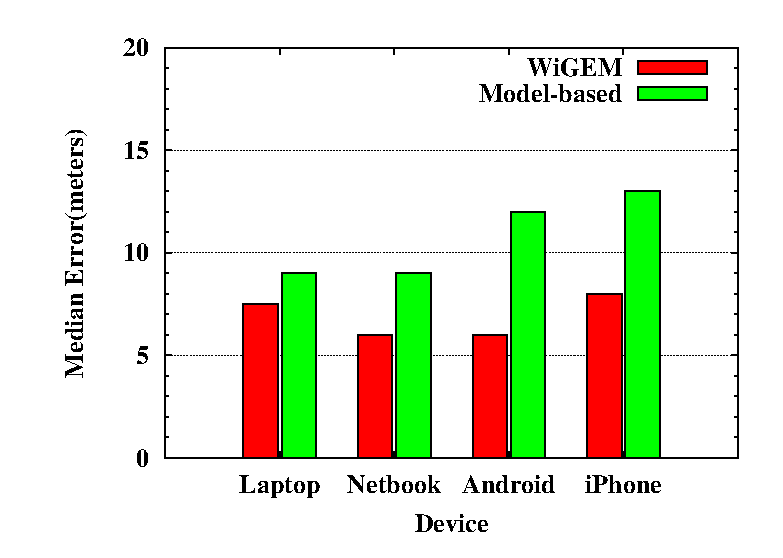
\includegraphics[height=1.5in, width=2.5in]{Figs4Paper/CEWIT/Baseline4Paper_CEWIT/BaselineComparisonsMedianError_cewit.eps}}
	      \subfloat[CSD]{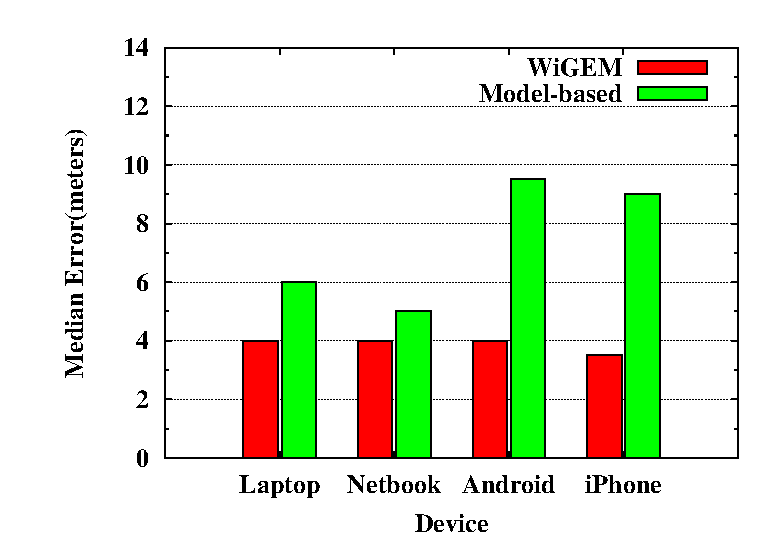
\includegraphics[height=1.5in, width=2.5in]
	      {Figs4Paper/CSD/Baseline4Paper_CSD/BaselineComparisonsMedianError_csd.eps}}
	\caption{Baseline Comparisons}
	\label{fig:baselinecomparisons}
\end{figure*}

% \begin{figure*}
% \begin{minipage}{0.5\textwidth}
% 	{\centering
% 	  \subfloat[Probabilistic]{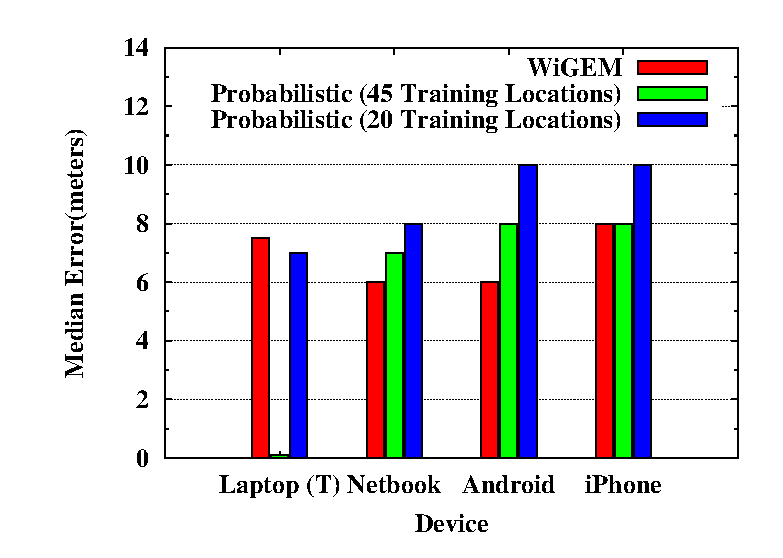
\includegraphics[width=0.5\textwidth]{Figs4Paper/CEWIT/HRComparisons4Paper_CEWIT/HRComparisonsMedianError_Probabilistic_cewit.eps}}
% 	  \subfloat[RADAR]{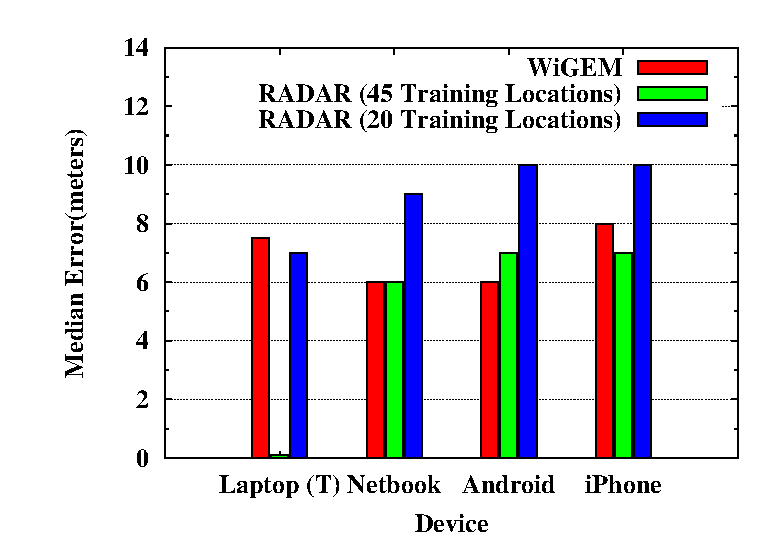
\includegraphics[width=0.5\textwidth]{Figs4Paper/CEWIT/HRComparisons4Paper_CEWIT/HRComparisonsMedianError_RADAR_cewit.eps}}
% 	\caption{Comparisons on the CEWIT Testbed}
% 	\label{fig:HR_on_cewittestbed}
% 	}
% \end{minipage}\quad
% \begin{minipage}{0.5\textwidth}
% 	{\centering
% 		\subfloat[Probabilistic]{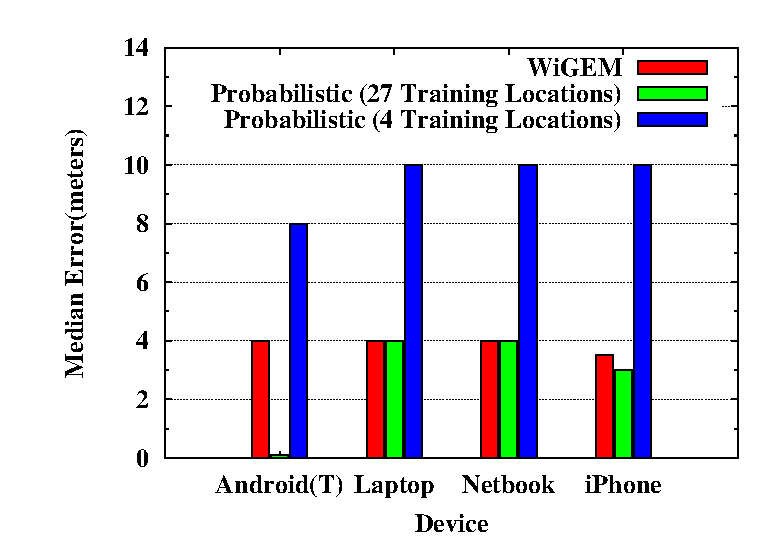
\includegraphics[width=0.5\textwidth]{Figs4Paper/CSD/HRComparisons4Paper_CSD/HRComparisonsMedianError_Probabilistic_csd.eps}}
% 		\subfloat[RADAR]{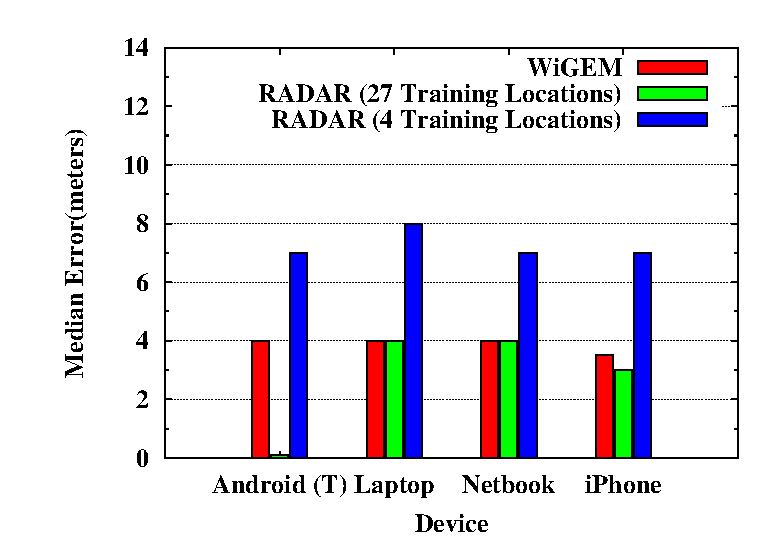
\includegraphics[width=0.5\textwidth]{Figs4Paper/CSD/HRComparisons4Paper_CSD/HRComparisonsMedianError_RADAR_csd.eps}}
% 	\caption{Comparisons on the CSD Testbed}
% 	\label{fig:HR_on_csdtestbed}
% 	}
% \end{minipage}
% \end{figure*}

Here we analyze the performance of GEM with respect to a model-based scheme that uses the indoor radio path loss propagation model (Section \ref{subsec:handlingidentifiabilityinourmodel}). This presents a true head-to-head comparison, because both the techniques do not need pre-deployment effort and can  give a location estimate at the same granularity of discretization of the target space. Both our testbeds, CEWIT and CSD, have been discretized as shown in Figure \ref{fig:experimenttestbed}. There are 267 grid vertices inside the CEWIT testbed roughly every 2.75 meters. The CSD testbed has 36 grid vertices roughly every 3.1 meters. GEM can localize a given target RSS vector to any of these grid vertices. As mentioned in Section \ref{subsec:datacollectionmethodology}, the data for our experimental evaluation is coming from 45 distinct locations on the CEWIT testbed and 27 distinct locations in the CSD testbed. There are 200 RSS tuples for every location on the map for each of the four device types. As mentioned above in Section aa, GEM is using a learning set size of 100 RSS samples with 45 power levels to build the model. Thus the test-set for both the algorithms is remaining 100 RSS tuples from each location. Each device type is evaluated separately.

The log-distance path loss (LDPL) mentioned in Section \ref{subsec:handlingidentifiabilityinourmodel} is used to estimate the RSS that should be observed at a sniffer for each grid vertex inside the target-space. These RSS values are used to initialize GEM, as mentioned in section \ref{subsec:handlingidentifiabilityinourmodel}. The Model-based algorithm also uses these same RSS values with a suitable metric to give a final location estimate. Similar to \cite{Bahl00radar:an}, the model-based algorithm that we use here uses nearest neighbor in signal space (NNSS) as the metric of choice. 

Figure \ref{fig:baselinecomparisons} shows the median error for both techniques. We see that GEM performs better than the model-based scheme across all device types in both the testbeds.

\subsection{Comparisons with schemes that use RF signal maps}
\label{subsec:comparisonswithschemesthatuserfsignalmaps}

\begin{figure*}
	\centering
	      \subfloat[Probabilistic]{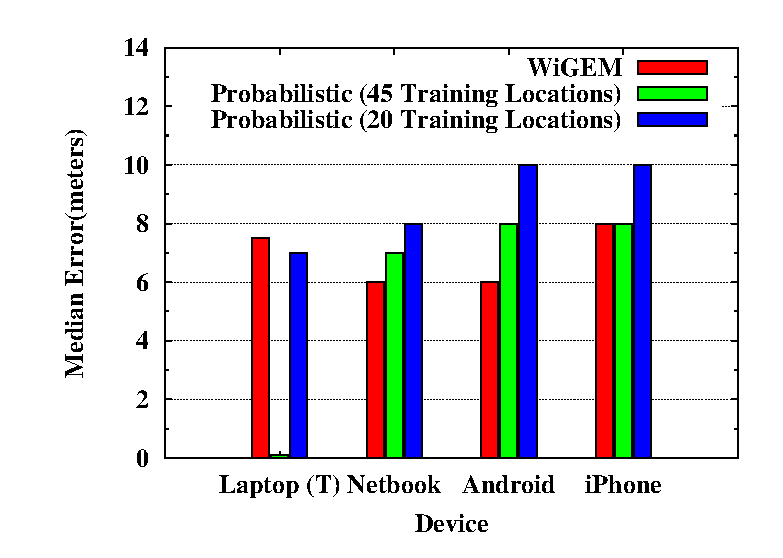
\includegraphics[height=1.5in, width=2.5in]{Figs4Paper/CEWIT/HRComparisons4Paper_CEWIT/HRComparisonsMedianError_Probabilistic_cewit.eps}}
	      \subfloat[RADAR]{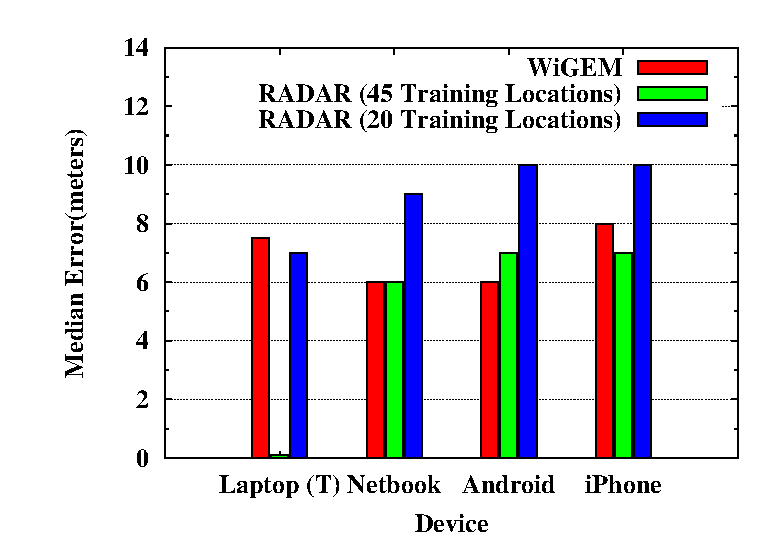
\includegraphics[height=1.5in, width=2.5in]
	      {Figs4Paper/CEWIT/HRComparisons4Paper_CEWIT/HRComparisonsMedianError_RADAR_cewit.eps}}
	\caption{Comparisons on the CEWIT testbed}
	\label{fig:HR_on_cewittestbed}
\end{figure*}

\begin{figure*}
	\centering
	      \subfloat[Probabilistic]{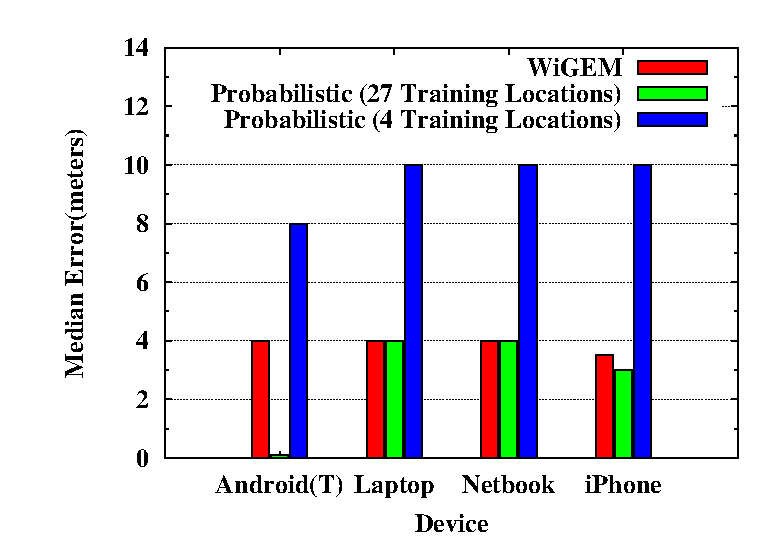
\includegraphics[height=1.5in, width=2.5in]{Figs4Paper/CSD/HRComparisons4Paper_CSD/HRComparisonsMedianError_Probabilistic_csd.eps}}
	      \subfloat[RADAR]{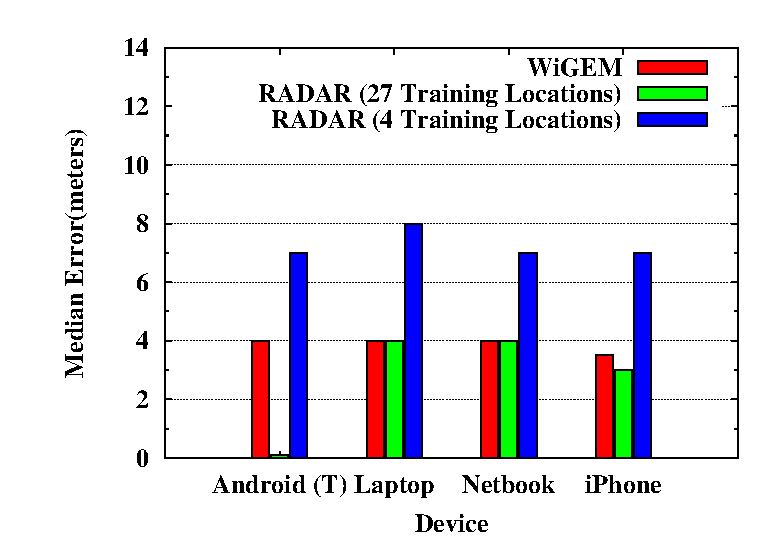
\includegraphics[height=1.5in, width=2.5in]
	      {Figs4Paper/CSD/HRComparisons4Paper_CSD/HRComparisonsMedianError_RADAR_csd.eps}}
	\caption{Comparisons on the CSD testbed}
	\label{fig:HR_on_csdtestbed}
\end{figure*}

We now compare the performance of GEM again two schemes that spend considerable pre-deployment effort in first building an RF signal map from RSS signatures collected from various locations inside the target space. Both schemes differ in the way they handle an incoming signature to provide a location estimate.

\begin{itemize}
\item Deterministic schemes like RADAR \cite{Bahl00radar:an} use the nearest neighbor in signal space (or an average of k-nearest neighbors) as the metric to give a location estimate. 
\item Probabilistic schemes \cite{Haeberlen:2004:PRL:1023720.1023728, Youssef:2008:HLD:1399551.1399558, Roos} on the other hand maintain a probability distribution of the RSS value from various locations. For the incoming signature, a probability distribution is built over the location space and a maximum likelihood estimate is used to determine position. As in \cite{Haeberlen:2004:PRL:1023720.1023728}, we model signal intensity as a normal distribution determined by the location and sniffer pair. 
\end{itemize}

\subsubsection{Discussion}
\label{subsubsec:rfsignalmapdiscussion}

\begin{enumerate}

\item 
For all three techniques that we compare here viz GEM, RADAR and Probabilistic, we consider the best location as our location estimate. We do not consider the weighted average of the top few locations for any of the three techniques compared here. 

\item
To show the WiFi hardware variance problem mentioned in Section \ref{sec:introduction}, we use different devices for location estimation. For the CEWIT testbed, a DELL Laptop was used to train the radio map during the {\it `offline' phase}. In the CSD testbed, an android phone was used to build the radio map. Based on the radio maps, four different device types are used to give location estimates. 

\item
As mentioned in Section \ref{subsec:datacollectionmethodology}, the data for our experimental evaluation is coming from 45 distinct locations on the CEWIT testbed and 27 distinct locations in the CSD testbed. 

For RADAR and Probabilistic, we try to understand the effect of the granularity of training locations on the final location estimate. We consider two scenarios : one optimistic and the other more realistic. In the first scenario, we consider the optimistic secnario where the training and test data sets (mentioned below) are collected at the same physical locations, e.g on the CEWIT testbed, the signal map is built from the same 45 distinct locations where the position estimation is being done. The second scenario, is the more realistic scenario where the training is done from only a subset of the test locations. Thus the testing locations are no longer strictly co-located with the training locations. In the CEWIT testbed, the training is done from 20 locations (out of the 45 possible) roughly every 10.3 meters apart. In the CSD testbed, the subset comprises of 4 locations (out of the 27 possible) roughly every 12.7 meters apart.  We note here that GEM on the other hand requires no training effort. For GEM we use the same discretization of the target space that we use in section \ref{subsec:baselinecomparisonwithamodelbasedscheme} i.e the GEM location estimate can be on any of the grid points inside the building.

\item
There are 200 RSS tuples for every location on the map for each of the four device types. We divide these 200 tuples into two disjoint sets of 100 tuples each. The first set is used by RADAR and Probabilistic to build their RF signal maps while GEM uses it as the learning data to build the localization model.  The second set of 100 tuples from each location is used as the test data for all three algorithms. Every device type is evaluated separately. 

\end{enumerate}

\begin{figure*}
	\centering
		\subfloat[CEWIT]{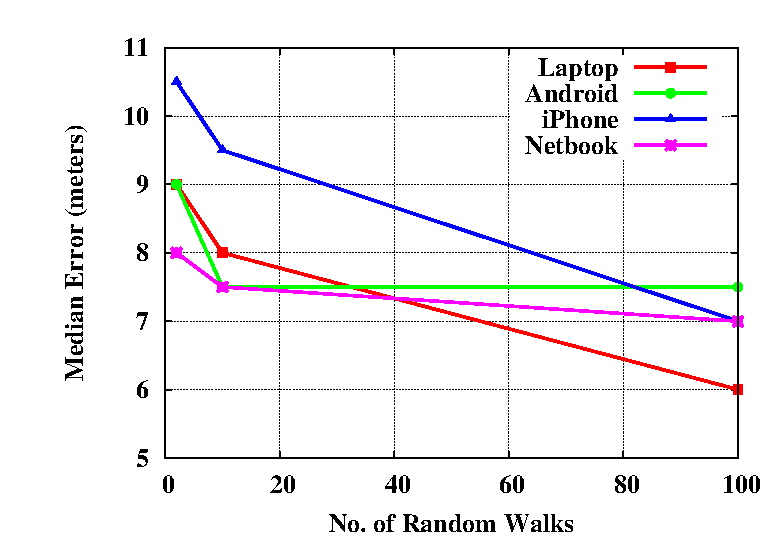
\includegraphics[height=1.5in, width=2.5in]{Figs4Paper/CEWIT/MobilityPlot4paper_CEWIT/Mobility_cewit.eps}}
		\subfloat[CSD]{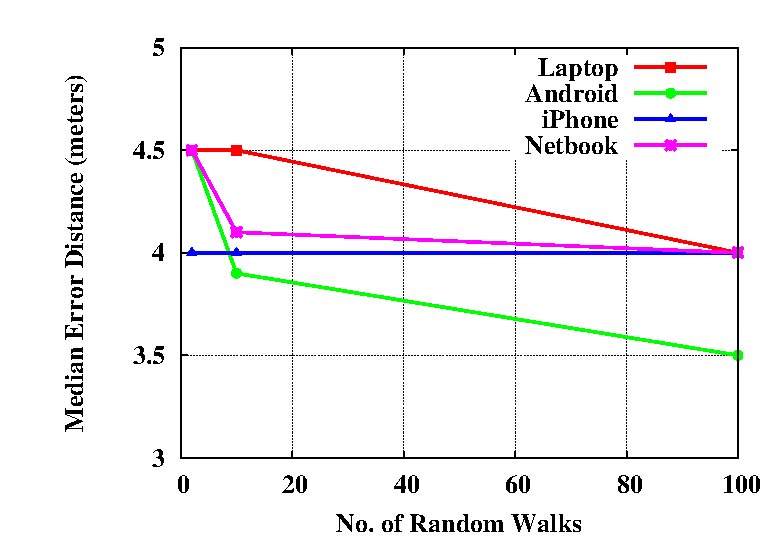
\includegraphics[height=1.5in, width=2.5in]{Figs4Paper/CSD/MobilityPlot4paper_CSD/Mobility_csd.eps}}
	\caption{Mobility}
	\label{fig:mobility}
\end{figure*}

\subsubsection{Observations}
\label{subsubsec:rfsignalmapobservations}

Figure \ref{fig:HR_on_cewittestbed} and Figure \ref{fig:HR_on_csdtestbed} shows the median error comparison between the three techniques . We make some interesting observations here:
 
\begin{itemize}

\item Hardware variance is a major issue for both RADAR and Probabilistic. When the same device is used for training and testing, the median error is zero. For other devices it jumps up dramatically. This is a critical problem for such techniques because a real-world deployment would be typically unaware of the device type being localized. In fact, we see GEM performing as good as RADAR and Probabilistic for other device types. This is particularly promising because unlike RADAR and Probabilistic, GEM did not have the overhead of a pre-deployment effort.

\item When the granularity of sampling is reduced, RADAR and Probabilistic start showing substantially poorer accuracy estimates. Thus location estimates for such techniques are tightly bound to the granularity of the training effort. This makes them unattractive for performing localization in large target spaces. A heavy pre-deployment effort also make these techniques difficult to maintain and  update in a dynamic environment.

\end{itemize}

\subsection{Impact of Mobility on GEM's localization accuracy}
\label{subsec:impactofmobilityongemslocalizationaccuracy}

In this experiment we try to understand how the mobility of a client can effect the location estimates made by GEM. To create the test data set, a user initially walks across all distinct location on the map, making 100 ping transmissions from each location. This forms our test data set which is basically a union of 100 RSS tuples from each distinct location on the map.  Now we try to observe the effect of client mobility in localizing this test data set. To do this, the user follows a random walk scheme. In each random walk, the user visits every distinct location in the building floor once, and makes a single ping transmission from that location. This serves as the learning data-set for GEM, in order to build a model for the device and give location estimates for the test set. 

We evaluate this scheme on both testbeds across four different devices. Figure \ref{fig:mobility} shows how the median error of the test data set varies as the mobility (i.e the number of random walks) increases. We observe that mobility actually helps GEM localization accuracy.


%\section{Discussions}
\label{sec:discussion}


In its current embodiment, WiGEM uses a radio propagation model (Section ~\ref{subsec:handlingidentifiabilityinourmodel}) for initializing the WiGMM model. For handling identifiability in our model, we exploit the typical constraints between the means of the Gaussians at the same location for different power levels. Future work can explore whether enforcing similar  constraints during run time increases the localization accuracy. Our framework could also be used to do a more efficient training process, whereby the radio propagation model is substituted by a few carefully done measurements. In this case, including the power of the source into the model may increase the robustness of the method and make it work for various devices. As future work, we also plan to do adaptive localization by doing learning and using the adjacency of the locations as information to track how motion could evolve. This seems to have been done with EM before~\cite{Addesso:2010:ALT:1856330.1856381} and might be nicely combined with our technique. Additional factors like the number and location of sniffers, the size of the grid etc., and their effect on localization accuracy can also be explored.
%1. Number of Sniffers and its impact. 
%
%2. Size of grid. Does finer grid work better ? 
%
%3. The same framework could also be used to do a more efficient training process. Basically, the model of Eq.(20) could maybe be substituted by a few carefully done measurements. The paper correctly identifies that such training works well for the device that performs the measurement but not for others. However, it seems that the inclusion of the power of the source in the model may increase the robustness of the method and make it work for various devices.
%[AG] This is actually  a 'strengthening' comment. Should we include this in the paper ?
%Yes. The model of Eq.(20) could maybe be substituted by a few carefully done measurements. . This is infact a strength of the proposed technique. We used  Eq.(20) instead to make our technique totally training-free. Future work can address the issue of how much benefit we get by initializing the model using a few carefully done measurements.
%
%[SRD] We can include this comment in the paper.
%
%4. 2.	There are typically constraints between the means of the Gaussians at the same location for different power levels. These constraints are enforced at initialization time when the means at a location for K power levels are initially set. But it is unclear how these constraints are enforced during the algorithm - so it seems possible that means for different transmit power levels at the same location may be quite far apart
%
%5. Paper lacks a statement of how to prevent the model from presenting bad solutions. A characterization of the error cases, and a discussion of what keeps the model in check, would be welcome.
%
%6. As the model uses unsupervised learning, a discussion of the nature of the errors and what could happen in degenerate situations would be welcome.
%
%7. I was a little disappointed that you didn't try tracking mobility by doing learning and using the adjacency of the locations as information to track how motion could evolve. I guess this could reduce the error further? This seems to have been done with EM before : Adaptive localization techniques in WiFi environments,    Paolo Addesso, Luigi Bruno, Rocco Restaino, ISWPC'10. and might be nicely combined with your technique




\section{Conclusions}
\label{sec:conclusions}

In this work, we have developed WiGEM, an infrastructure based technique to localize a
wireless client in an indoor environment based on the RSS
 of its transmitted packets as received by a sniffer (or an AP doubling 
as sniffer). WiGEM is based on a learning-based
algorithm that can learn the parameters of a Gaussian Mixture Model
dynamically from packets captured by the sniffers.
By using dynamic packet captures for parameter
estimation, WiGEM can provide location estimates 
that are much more robust in the face of device and power level
variabilities, mobility, and changes
and reconfiguration of indoor spaces that many training-based systems
are susceptible to. The biggest advantage of WiGEM is that there is no explicit 
training phase. This saves a significant pre-deployment effort that is also
difficult to maintain and update. Performance evaluations with 
a range of different WiFi devices in two different indoor testbeds demonstrate
that WiGEM performs better than model-based techniques and at par or better than 
state-of-the-art RF map-based techniques. Of particular importance is WiGEM's
superior performance when heterogeneous devices are used and when the RF map-based
techniques have coarser training locations. 


%{\bf Infact, we showed that we can achieve accuracy that is at par with state-of-the-art
%techniques that use training to build RF-signal maps first} Thus,
%our technique not only eliminates the intensive time-consuming (often manual) training phase
%but also makes our technique scalable for large target spaces.
%
%\section{Placeholder. BibRef. (To Remove)}
% Haeberlen04 \cite{Haeberlen:2004:PRL:1023720.1023728},
% Gwon04 \cite{Gwon:2004:ECC:1023783.1023786},
%Elnahraway04 \cite{Elnahraway:2004:LLU:1031495.1031537},
% Moraes06 \cite{Moraes:2006:CWL:1164783.1164799},
% Youssef08 \cite{Youssef:2008:HLD:1399551.1399558},
%Ferris07 \cite{Ferris:2007:WUG:1625275.1625675},
%Berna03 \cite{Berna:2003:LAL:1630659.1630885},
% Lim10 \cite{Lim:2010:ZIL:1741400.1741464},
% Tsui09 \cite{Tsui:2009:ULS:1741410.1741596},
% Chintalapudi10 \cite{Chintalapudi:2010:ILW:1859995.1860016},
% Ladd02 \cite{Ladd:2002:RLS:570645.570674},
% Youssef03 \cite{Youssef:2003:WLD:826025.826335},
% Tao03 \cite{Tao:2003:WLL:941311.941314},
% Krishnan04 \cite{Krishnan04asystem},
% Borman \cite{Borman_theexpectation},
% Bilmes97 \cite{Bilmes97agentle},
%Roos02 \cite{Roos},
% Madigan \cite{Madigan05bayesianindoor},
% Bahl00 \cite{Bahl00radar:an},
% Molkdar91 \cite{Molkdar},
% Bishop \cite{Bishop:2006:PRM:1162264},
% Reynolds \cite{Reynolds},
%Dempster77 \cite{Dempster77maximumlikelihood},
%Dinov \cite{DinovIvoD},
%Rappaport \cite{Rappaport:2001:WCP:559977}


\bibliographystyle{abbrv}
\bibliography{sigproc}  

\end{document}  

